%===============================================================================
% OBDH laboratory manual
%
% (C) 2020 Juan A. de la Puente <juan.de.la.puente@upm.es>
% (C) 2022 Juan Zamorano <juanrafael.zamorano@upm.es>
% (C) 2023 Ángel-Grover Pérez-Muñoz <angel.perez.munoz@upm.es>
%
% Some rights reserved. This work is licensed under a  
% Creative Commons Attribution-NonCommercial-ShareAlike 4.0 International License.
% http://creativecommons.org/licenses/by-nc-sa/4.0/
%===============================================================================
\documentclass[12pt,a4paper,english,twoside]{book}

\bibliographystyle{abbrvnat}
\usepackage{natbib}

\usepackage[utf8]{inputenc}    % UTF8 encoding
%\usepackage{t1enc}            % Latin1 characters
%\usepackage{babel}            % hyphenation etc. - not needed 
\usepackage{graphicx}          % figures
\DeclareGraphicsExtensions{.pdf,.png,.jpg}
\graphicspath{{fig/}}
\usepackage{xcolor}

\usepackage{amssymb,amsmath}
\usepackage{alltt}
\usepackage[hmargin=3cm,vmargin=2cm]{geometry} % page margins
\usepackage{calc}
%\usepackage[lineno5]{lgrind}
\usepackage{hyperref}
%\usepackage{fontspec,xunicode,xltxtra}
\usepackage{gensymb}
\usepackage{float}
\usepackage{theorem}
\usepackage{listings}

%\usepackage{indentfirst} % Indent 1st paragraph
\usepackage{parskip}
\usepackage{fancyvrb}

\usepackage{tcolorbox}

\usepackage{todonotes}
\setlength{\marginparwidth}{2.5cm} % so that todonotes fit in a page

\definecolor{mGreen}{rgb}{0,0.6,0}
\definecolor{mGray}{rgb}{0.5,0.5,0.5}
\definecolor{mPurple}{rgb}{0.58,0,0.82}
%\definecolor{mPurple}{rgb}{101, 41, 128}
\definecolor{backgroundColour}{rgb}{255,255,255}
\definecolor{mRedBrown}{RGB}{168, 10, 10}
\definecolor{mOrangered}{RGB}{239,134,64}

%\lstset{inputpath=code/}
%\lstdefinestyle{CStyle}{
	%    backgroundcolor=\color{backgroundColour},
	%    commentstyle=\color{mGreen},
	%    keywordstyle=\color{magenta},
	%    numberstyle=\tiny\color{mGray},
	%    stringstyle=\color{mPurple},
	%    basicstyle=\footnotesize,
	%    breakatwhitespace=false,
	%    breaklines=true,
	%    captionpos=b,
	%    keepspaces=true,
	%    numbers=left,
	%    numbersep=5pt,
	%    showspaces=false,
	%    showstringspaces=false,
	%    showtabs=false,
	%    tabsize=4,
	%    morekeywords={vTaskNotifyGiveFromISR},
	%    language=C
	%}

%\lstdefinestyle{c}{
	%       language=c,
	%       basicstyle=\sffamily,
	%       xleftmargin=\parindent,
	%       numbers=none,
	%       columns=flexible,
	%}

%------------- software versions ------------------------------------

%\newcommand{\simplicitystudio}{Simplicity
	%Studio\textsuperscript{\tiny\texttrademark} 4 }
%\newcommand{\sdk}{Flex Software Development Kit (SDK) Gecko v5.0.0}
%\newcommand{\matlabversion}{Matlab R2018b}
%\newcommand{\gccversion}{\prog{GCC~7.2.1}}
%\newcommand{\gdbversion}{\prog{GDB~8.0}}
%\newcommand{\binutils}{\prog{binutils 2.29.51}}
%\newcommand{\newlibversion}{\prog{Newlib~2.5.0}}

%-------------- other commands ---------------------------------------
\newcommand{\prog}[1]{\textsf{#1}}

\newcommand{\program}[1]{{\ttfamily\upshape #1}}
\newcommand{\variable}[1]{{\slshape #1}}

%\newcommand{\prog}[1]{\texttt{#1}}

\theoremstyle{break}\newtheorem{warning}{WARNING}[chapter]

\newenvironment{entry}[1]
{\begin{list}{}%
		{\renewcommand{\makelabel}[1]{\textbf{##1}\hfil}%
			\settowidth{\labelwidth}{\textbf{#1}}%
			\setlength{\leftmargin}{\labelwidth+\labelsep}%
		}%
	}%
	{\end{list}}

%\renewcommand{\CMfont}{\ttfamily\slshape}
%\renewcommand{\KWfont}{\ttfamily\bfseries}
%\renewcommand{\VRfont}{\ttfamily\upshape}
%\renewcommand{\BGfont}{\ttfamily\upshape}

%\renewcommand{\LGnuminterval}{1}

%======================= document ===================================
\begin{document}
	%======================= front matter ===============================
	\frontmatter
	
	%!TEX root = practica.tex
%===============================================================================
\begin{titlepage}

%\begin{center}
%\framebox{
%\begin{minipage}{100mm}
%\begin{center}
%\textbf{STRAST/UPM}
%\end{center}
%This report describes the second laboratory assignment of Data Handling course.
%\end{minipage}
%}
%\end{center}

%\includegraphics[height=20mm]{MUSE}\hfill

\includegraphics[height=20mm]{UPM}


\vfill\vspace{50pt}

\begin{center}
%\rule{\textwidth}{1pt}\\[2\baselineskip]
\textbf{\huge Sistemas Empotrados y Ubicuos}\\[\baselineskip]
{\large Máster Universitario en Ingeniería Infórmatica}\\[\baselineskip]
\textbf{\Huge Cross-Development Environment Work}\\[\baselineskip]
{\large Version 1.2 --- \today}\\[\baselineskip]
{\large\textsc{1st student assignment}}
\end{center}

\vfill

\begin{center}\textsc{
\rule{\textwidth}{1pt}\\
Universidad Politécnica de Madrid\\
DATSI\\
Departamento de Arquitectura y Tecnología de Sistemas Informáticos\\}
\url{https://www.datsi.fi.upm.es}\\[1em]
\rule{\textwidth}{1pt}\\
\end{center}

\end{titlepage}

	\thispagestyle{empty}
	
	%!TEX root = practica.tex
%===============================================================================
{\footnotesize
\noindent
\copyright\ 2024 DATSI/UPM.

%\vspace{\baselineskip}\noindent
%Published by
%\begin{quote}
%Grupo STRAST\\
%Sistemas de Tiempo Real y Arquitectura de Sistemas Telemáticos\\
%%\url{https://www.dit.upm.es/str}\\
%Universidad Politécnica de Madrid\\
%Madrid\\
%SPAIN
%\end{quote}

\vspace{\baselineskip}
%Permission is granted to make and distribute verbatim copies of this
%manual provided the copyright notice and this permission notice are
%preserved on all copies.
%
%Permission is granted to copy and distribute modified versions of this
%manual under the conditions for verbatim copying, provided also that
%the sections entitled  Copying  and  GNU General Public License  (see
%appendix \ref{ap:licence}) are included exactly as in the
%original, and provided that the entire resulting derived work is
%distributed under the terms of a permission notice identical to this
%one.
%
%Permission is granted to copy and distribute translations of this
%manual into another language, under the above conditions for modified
%versions, except that this permission notice may be stated in a
%translation approved by the Free Software Foundation.
\noindent

\includegraphics{cc-by-nc-sa-4_0.png}

\noindent
This work is licensed under a Creative Commons Attribution-NonCommercial-ShareAlike 4.0 International License.
 \url{https://creativecommons.org/licenses/by-nc-sa/4.0/}

%\vspace{\baselineskip}
%\noindent
%\begin{tabular}{lp{120mm}}
%\textbf{Status:}  & Ongoing\\
%\\
%\textbf{Authors:}    & Juan Antonio de la Puente\\
%                     & Juan Zamorano\\
%\\
%\textbf{Revised by:} & Juan Zamorano\\
%\end{tabular}
%
%\vspace{2\baselineskip}
%\noindent
%\begin{tabular}{llp{120mm}}
%\textbf{History}\\
%\textbf{Version}&\textbf{Date}&\textbf{Comments}\\
%\end{tabular}
%
%}







	\cleardoublepage\pagestyle{plain}
	%\pagenumbering{roman}
	\setcounter{page}{1}
	\setcounter{tocdepth}{1}
	\tableofcontents
	
	%======================= document body =================================
	\mainmatter
	\cleardoublepage
	\pagestyle{headings}
	\pagenumbering{arabic}\setcounter{page}{1}
	%----------------------------------------------------------------------
	%!TEX root = practica.tex
%===============================================================================
\chapter*{Introduction}\label{ch:introduction}
\addcontentsline{toc}{chapter}{Introduction}
%----------------------------------------------------------------------

This document provides instructions for laboratory work in the field of embedded systems. The laboratory is part of the Embedded and Ubiquitous Systems course of the UPM's Máster Universitario en Ingeniería Infórmatica (MUII) program.
The laboratory is based on a computer kit that is used to build a simplified version of a satellite on-board software system (OBSW). An instance of the laboratory kit will be made available to every student registered in the course during the laboratory session.

Students are required to use their own personal computer, running Windows, MacOS, or GNU/Linux, to carry out the laboratory assignments. 
The outline of the laboratory assignments is as follows:
\begin{enumerate}
\item	Installation of a native programming environment.
\item	Installation of the cross-platform programming tools.
\item   On-board data handling (OBDH) system.
\item   OBDH system with Attitude Control System (ACS).
\end{enumerate}

%----------------------------------------------------------------------
\section*{References}
\addcontentsline{toc}{section}{References}

The following documents contain additional information about the software
and hardware tools used to develop the work:

\subsection*{Hardware}
\begin{enumerate}
\item	\href{https://www.st.com/resource/en/data\_brief/stm32f4discovery.pdf}{STMicroelectronics. DB1421 Data Brief.  STM32F4DISCOVERY - Discovery kit with STM32F407VG MCU.}

\item \href{https://www.st.com/content/ccc/resource/technical/document/user\_manual/70/fe/4a/3f/e7/e1/4f/7d/DM00039084.pdf/files/DM00039084.pdf/jcr:content/translations/en.DM00039084.pdf}{STMicroelectronics. UM1472 User manual - Discovery kit with STM32F407VG MCU.}

\item \href{https://www.st.com/resource/en/datasheet/dm00037051.pdf}{STMicroelectronics. DS 8626. Data sheet - STM32F405xx, STM32F407xx. ARM Cortex-M4 32b MCU+FPU, 210DMIPS, up to 1MB Flash/192+4KB RAM, USB OTG HS/FS, Ethernet, 17 TIMs, 3 ADCs, 15 comm. interfaces \& camera.}

\item \href{https://www.st.com/content/ccc/resource/technical/document/reference\_manual/3d/6d/5a/66/b4/99/40/d4/DM00031020.pdf/files/DM00031020.pdf/jcr:content/translations/en.DM00031020.pdf}{STMicroelectronics. RM0090 Reference manual - STM32F405/415, STM32F407/417, STM32F427/437 and STM32F429/439 advanced Arm\copyright-based 32-bit MCUs.}
\end{enumerate}

\subsection*{Software}

\begin{enumerate}
\item \href{https://www.upm.es/sfs/Rectorado/Vicerrectorado\%20de\%20Tecnologias\%20de\%20la\%20Informacion\%20y\%20Servicios\%20en\%20Red/Servicio\%20de\%20Planificacion\%20Informatica\%20y\%20Comunicaciones/SW/MATLAB\_UPM\_Estudiantes.pdf}{Access and installation procedure of MATLAB for UPM students.}

\item \href{http://www.ada-auth.org/standards/rm12i\_w\_tc1/html/RM-TTL.html}{Ada Reference Manual.}

\item	GNAT User's Guide for Native Platforms.

\item	GNAT User's Guide Supplement for Cross Platforms

\item	GNAT Reference Manual.
\end{enumerate}

%----------------------------------------------------------------------

\section*{Acronyms}
\addcontentsline{toc}{section}{Acronyms}

\begin{entry}{RAVENSCAR}
\item[ADC] Analog to Digital Converter.
\item[ACS] Attitude Control System.
\item[DAC] Digital to Analog Converter.
\item[FPU] Floating Point Unit.
\item[GCC] GNU compilation system..
\item[GDB] GNU Debugger.
\item[GNAT] GNU Ada Translator.
\item[GNU] GNU is not Unix.
\item[GPL] GNU Public License.
\item[GPS] GNAT Programming Studio.
\item[LGPL] Lesser GNU Public License (formerly Library GPL).
\item[MCU] Microcontroller Unit.
\item[OBC] On-Board Computer.
\item[OBDH] On-Board Data Handling.
\item[OBSW] On-Board Software.
\item[OS] Operating System.
\item[PC] IBM Personal Computer architecture.
\item[TC] Telecommand.
\item[TM] Telemetry.
\item[USART] Universal Synchronous Asynchronous Receiver Transmitter.
\item[USB] Universal Serial Bus.
\end{entry}


	%!TEX root = practica.tex
%===============================================================================
\chapter*{Overview}\label{ch:overview}
\addcontentsline{toc}{chapter}{Overview}
%----------------------------------------------------------------------

\section*{Laboratory kit components}
\addcontentsline{toc}{section}{Laboratory kit components}

The laboratory kit includes:
\begin{itemize}
\item	An STM32F407 computer board that emulates an on-board computer (OBC) system.

\item	A USB A / mini USB cable that is used to connect the OBC to the development station hosted on the student PC.

\item	A USB / UART interface cable that is used to provide a serial line link between the OBC board and the ground station software running on the student PC.
\end{itemize}

The figure~\ref{fig:kit} shows the components of the laboratory kit and the connections to a PC.

\begin{figure}[h]
            \centering{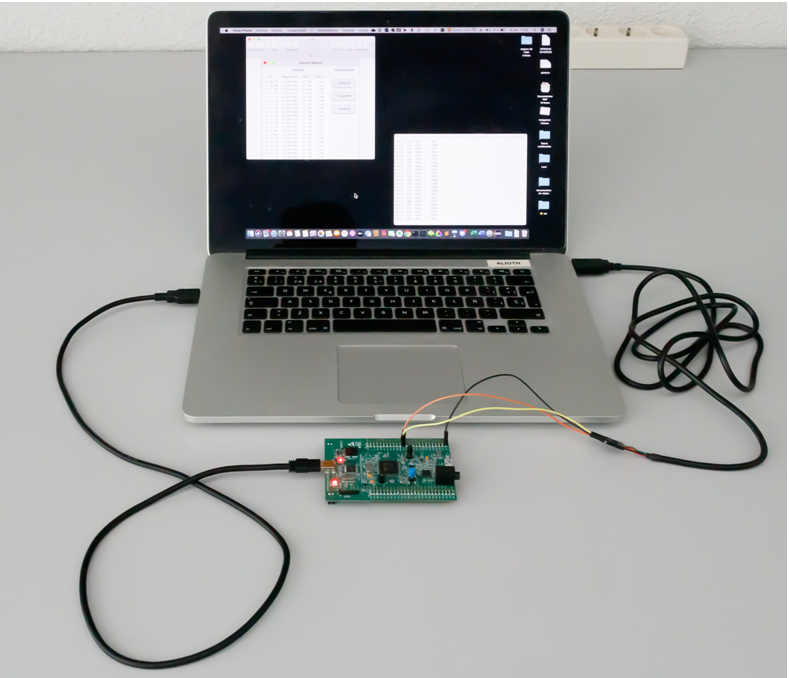
\includegraphics[width=.6\textwidth,keepaspectratio]{laboratory_kit.png}}
            \caption{Laboratory kit.}
            \label{fig:kit}
\end{figure}

\section*{Architecture of the laboratory system}
\addcontentsline{toc}{section}{Architecture of the laboratory system}

The figure~\ref{fig:architecture} depicts the architecture of the laboratory system which consists of two segments.
The \textit{flight segment} is deployed on the laboratory computer board,
and, the \textit{ground segment} is deployed on the student's PC.
The communication between both segments is carried out by means of a serial line,
simulating the radio link of a real satellite mission.
The student's work is centered on programming the computer board.
The ground station software will be provided by the professors.

\begin{figure}[hbtp!]
            \centering{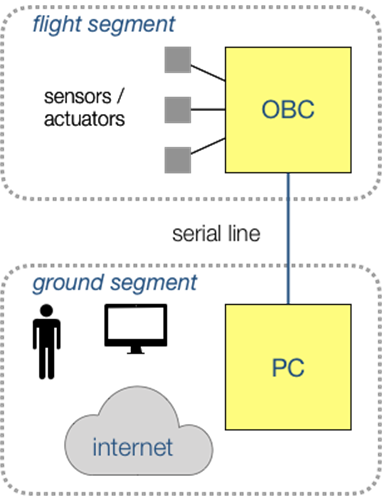
\includegraphics[width=0.35\textwidth,keepaspectratio]{architecture.png}}
            \caption{Architecture of the laboratory system.}
            \label{fig:architecture}
\end{figure}

\section*{Computer board and connections}
\addcontentsline{toc}{section}{Computer board and connections}

The STM32F407 board is used as a low-cost replacement for a satellite OBC.
The board features a 32-bit ARM Cortex-M4 microcomputer,
192 KB of RAM, 1 MB of Flash memory and a number of embedded devices.
The figure~\ref{fig:board}
\todo{Mejorar definición de la imagen y resaltar los pines}
shows an overall view of the computer board.

\begin{figure}[h]
    \centering{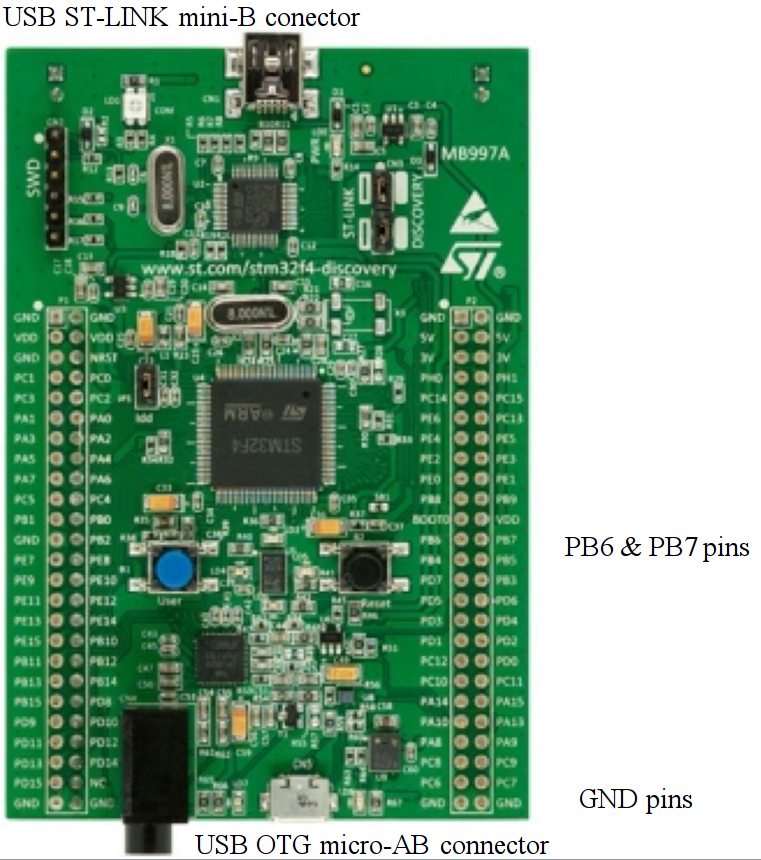
\includegraphics[height=10cm,keepaspectratio]{board.png}}
    \caption{Computer board.}
    \label{fig:board}
\end{figure}

The following are the main components used in this laboratory:
\begin{itemize}
\item	USB ST-LINK connector, which is linked to a PC with a mini-USB to USB-A cable. This connection is used to supply power to the board (5 V) and load and debug the software from the host PC.

\item	General Purpose Input-Output (GPIO) pins PB6, PB7 and GND.
GPIO is a standard interface for connecting external devices.
These GPIO pins are used in the laboratory
to connect a serial line to a USB port on a PC,
emulating the connection to the on-board radio equipment in a satellite.
Specifically the pin:
\todo{RX and TX pins?}
\begin{itemize}
	\item \textbf{PBX} is used as the receiver pin (RX).
	\item \textbf{PBY} is used as the transmitter pin (TX).
	\item \textbf{GND} is used for grounding.
\end{itemize}

\item	Temperature and voltage sensors. These sensors are part of the STM32 microcomputer chip,
and can be read using internal registers in the MCU.
They are used in the laboratory to emulate the housekeeping devices onboard the satellite.
\end{itemize}

	\renewcommand{\chaptername}{Assignment}
	%!TEX root = practica.tex
%===============================================================================
\chapter{Set up}\label{ch:Setup}
\addcontentsline{toc}{chapter}{Set up}
%----------------------------------------------------------------------


\section{Install a native programming environment}
\addcontentsline{toc}{section}{Install a native programming environment}

The aim of this assignment is to
install a native programming environment
for the Ada language on the student's PC.
This environment will later be extended with cross-compilation tools
for the STM32 board to be used in the laboratory.

The programming environment is the GNAT Community version,
an open-source software development environment freely available from AdaCore,
a company specialized in providing tools
and solutions for developing high-integrity software.

% -- GNAT -----------------------------------------------------------------------

\subsection{Download and install GNAT}
The GNAT Community compilation system can be downloaded from \url{https://www.adacore.com/download/more}.
Installation packages for Windows, MacOS and GNU Linux
are available at the download page.
The file \texttt{README.txt} provides installation instructions,
which are summarized in the following subsections:

\subsubsection*{Windows}
\begin{enumerate}
\item Download the file \href{https://community.download.adacore.com/v1/797dbae8bdb8a3f661dad78dd73d8e40218a68d8?filename=gnat-2021-20210519-x86\_64-windows64-bin.exe\&rand=1472}{\texttt{gnat-2021-20210519-x86\_64-windows64-bin.exe}}

\item Run the file and follow the instructions.
\end{enumerate}

\textbf{\textcolor{mRedBrown}{Important}}:
GNATStudio installs additional configuration files in the \texttt{.gnatstudio} folder,
which is located under your Home directory (e.g.: \texttt{C:\textbackslash{}\textbackslash{}user\_name\textbackslash{}.gnatstudio}).
Notice that the application will not start if your user account contains special character such as spaces or accent marks.
Then, to solve this you must remove all special characters from your user account.
This 
\href{https://superuser.com/questions/890812/how-to-rename-the-user-folder-in-windows-10/1346983#1346983}
{link}
provides detailed instructions to solve this issue.

\subsubsection*{MacOS}
\begin{enumerate}
\item Download the file \texttt{gnat-2020-20200818-x86\_64-darwin-bin.dmg}
\item Open the dmg disk and execute the application inside it.
In order to circumvent the system protection,
control-click on the file and then click on ``opens" in the emergent window.
\end{enumerate}

Notice that you need to have installed the Xcode application to install GNAT.
If you still see the following error:

\begin{BVerbatim}
	ld: library not found for -lSystem
\end{BVerbatim}
\\

then you might have to execute the following:

\begin{BVerbatim}
	xcode-select -s /Applications/Xcode.app/Contents/Developer
\end{BVerbatim}

\subsubsection*{GNU Linux}
\begin{enumerate}
\item Download the file \texttt{gnat-2021-20210519-x86\_64-linux-bin}
\item You will need provide execution permissions to the binary in order to run it.
Run the following command in your terminal:

\begin{BVerbatim}
     chmod +x path_to_the_package.bin
\end{BVerbatim}

and execute the package. The \texttt{README.txt} file
contains additional installation and execution instructions.
\end{enumerate}

\subsection{Test the installation with a simple program}

The GNAT compilation system includes the
GPS (GNAT Programming Studio) integrated development environment,
which allows users to edit, compile, and run Ada and C programs. Figure\ref{fig:gps} shows the main GPS window,
which is composed of the following areas:

\begin{figure}[hbtp!]
    \centering{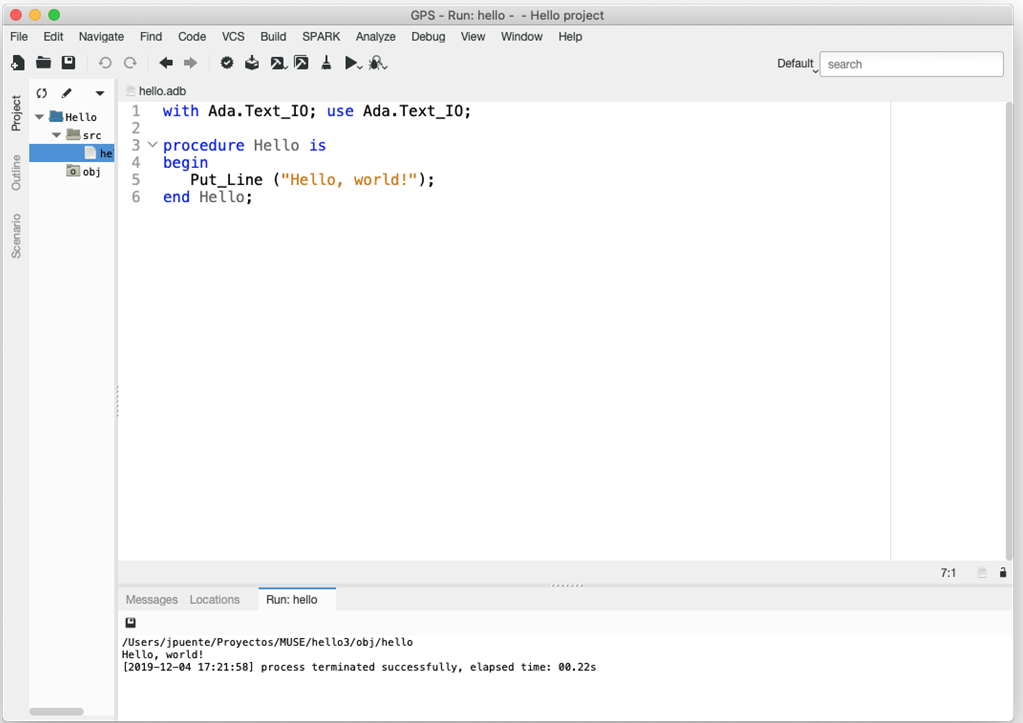
\includegraphics[width=\textwidth,keepaspectratio]{gps.png}}
    \caption{GNAT Programming Studio (GPS).}
    \label{fig:gps}
\end{figure}

\begin{itemize}
\item	a menu bar at the top
\item	a tool bar under the menu bar
\item	on the left, a notebook allowing you to switch between Project, Outline and Scenario views
\item	the working area in the center
\item	the messages window at the bottom
\end{itemize}

GPS organizes source code in projects.
A project is a set of source files which are compiled together
in order to produce a single binary executable.
Before starting you will need to create a folder to store your software projects.
The recommendation is to create a folder named
\textcolor{mPurple}{\texttt{SEU-OBDH-Lab}}
in the location of your choice.

The next activity consists on writing and running a simple Ada program with GPS:
\begin{enumerate}
\item 	Create a new project by clicking on File $\rightarrow$ New Project ...
        in the top menu. Choose the Simple Ada Project template.

\item	Choose a folder to deploy the project, e.g. \textcolor{mPurple}{\texttt{SEU-OBDH-Lab/lab-1}}.
        Set the project's name to \texttt{Hello} and the main name also to \texttt{Hello}.
        
\item	Double click on the \texttt{hello.adb} file in the project view to open the file in the working area.

\item	Edit the file in the working area so that it has the same content as in figure~\ref{fig:gps}.

\item	Build and run the executable by clicking on the $\rhd$ symbol in the tool bar.
You should see a number of compilation-related messages and,
if everything is right, you will see the text \texttt{Hello, world!}
in the Run tab of the bottom window.
\end{enumerate}
%\begin{figure}[h]
%            \centering{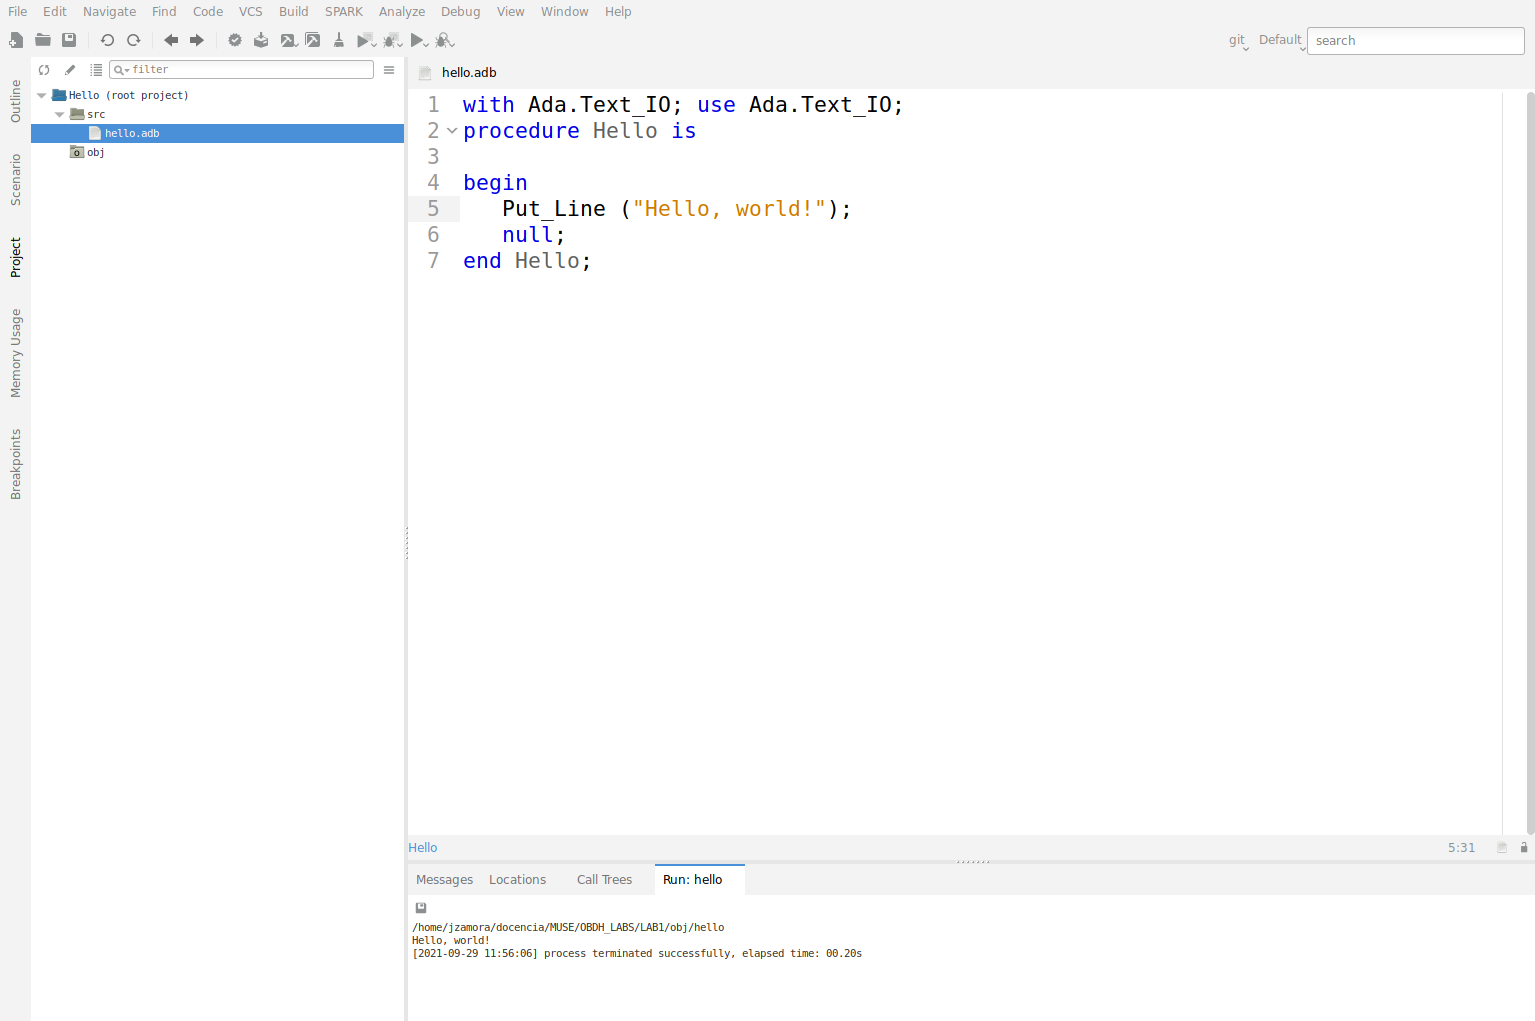
\includegraphics[width=\textwidth,keepaspectratio]{gpshello.png}}
%            \caption{Hello world demo program.}
%            \label{fig:gpshello}
%\end{figure}

\section{Install the cross-compilation tools}
\addcontentsline{toc}{section}{Install the cross-compilation tools}

The aim is to get acquainted with the embedded computer board
and to install and test the cross-compilation tools for GNAT
that will be used to develop executable code for it.

\subsection{Cross-compilation tools}

The computer board will programmed in Ada,
a systems programming language suitable for high-integrity applications.
The GNAT cross-platform development system
will be used to compile the software in the student's PC (aka. the host platform)
so that it can be uploaded in the SMT32 board (the target platform).

\begin{figure}[hbtp!]
    \centering{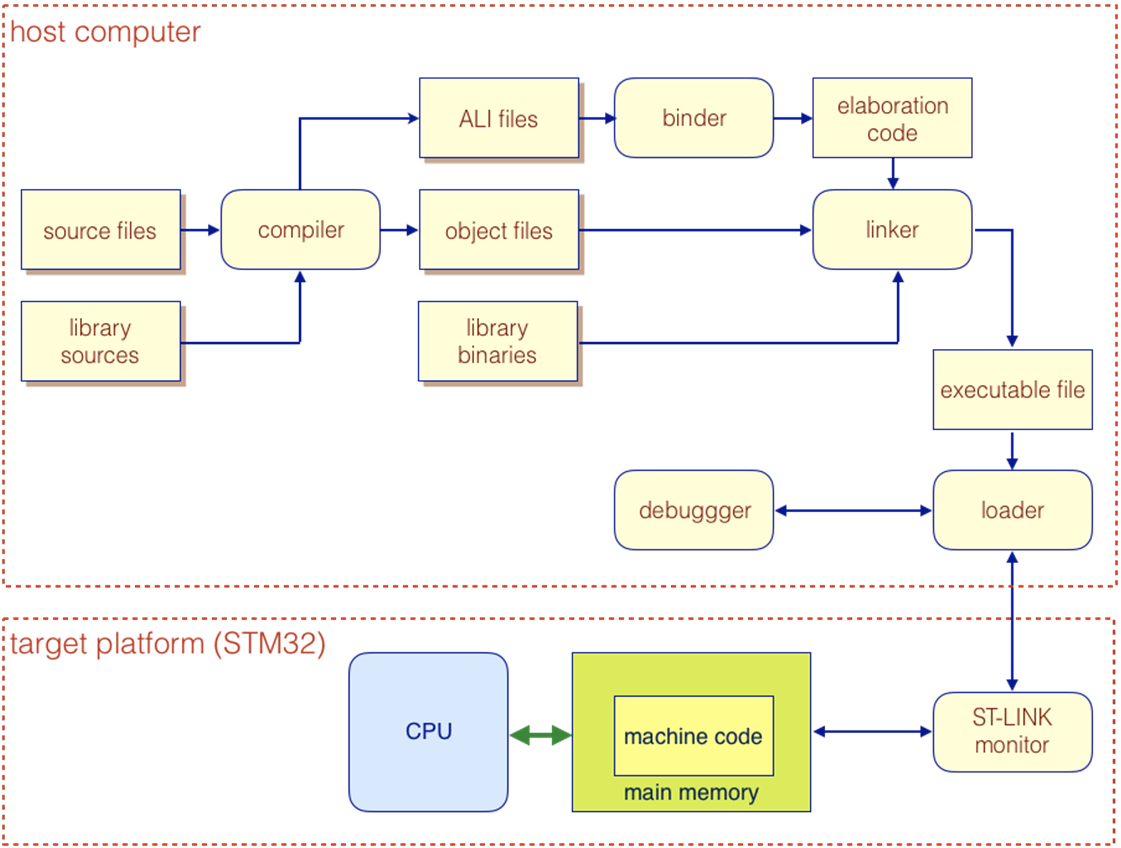
\includegraphics[width=\textwidth,keepaspectratio]{cross.png}}
    \caption{Cross-compilation and debugging system}
    \label{fig:cross}
\end{figure}

In order to compile a program, the compilation chain is run on the host computer to produce an executable file suitable for the target computer.
The executable is then loaded into the target memory,
from where it can be executed.
A monitor program is preinstalled on the target board
that supports loading and debugging from the host platform.

\subsection{Download and install GNAT ARM ELF}

GNAT ARM ELF is the cross-compilation chain to be used with the STM32F4 board. It can be downloaded from the
\href{https://www.adacore.com/download/more}{same page as the native GNAT system},
and there are installation packages for Windows, MacOS and GNU Linux available.
The file \texttt{README.txt} provides installation instructions,
which are summarized as follows.

\subsubsection*{Windows}
\begin{enumerate}
\item Select the platform ARM ELF (hosted on windows64) 2021, and download the file
gnat-2021-20210519-arm-elf-windows64-bin.exe
\item Run the file and follow the instructions.
\item You will also need to install the USB driver for the ST-LINK probe. To do so, go to \url{http://www.st.com/content/st\_com/en/products/embedded-software/development-tool-software/stsw-link009.html}, and click on Get Software. Click on Get Software under the Download column of the table that shows up to obtain the driver. You will need to accept ST Micro’s license agreement and enter your contact details. 
Once downloaded unzip the USB device driver and run the installer, accepting all the defaults.
\end{enumerate}
\subsubsection*{MacOS}
\begin{enumerate}
\item Select the platform ARM ELF (hosted on darwin) 2021, and download the file gnat-community-2019-20190517-arm-elf-darwin-bin.dmg
\item Open the dmg disk and execute the application inside it. In order to circumvent the system protection, control-click on the file and then click on ``open" in the emergent window.
\item You will also need the st-util,  st-flash, and st-info tools. You can download the binaries from 
\url{https://github.com/texane/stlink/releases/download/1.3.0/stlink-1.3.0-macosx-amd64.zip}. Unzip and copy the files in the bin directory to a directory in your PATH. You may need to circumvent MacOS protection by executing the command:

	\$ xattr -d com.apple.quarantine path-to-executable-file
\end{enumerate}
\subsubsection*{GNU Linux}
\begin{enumerate}
\item Select the platform ARM ELF (hosted on linux) 2021, and download the file gnat-2021-20210519-arm-elf-linux64-bin
\item You will need to make the package executable before running it. In a command prompt, execute the following command:

     chmod +x path\_to\_the\_package.bin

and then execute the package.
\item You will also need to install the stlink tools. In Ubuntu and Debian stlink must be installed from sources. Follow the instructions on \url{http://docs.adacore.com/live/wave/gnat\_ugx/html/gnat\_ugx/gnat\_ugx/arm-elf\_topics\_and\_tutorial.html\#linux}.
\end{enumerate}

The README.txt file contains additional installation and execution instructions.

\subsection{Test your installation with an embedded program}

The next activity is to compile and run a simple embedded program.
This program is only intended to test that the compilation chain
and the ST-LINK tools have been properly installed.

Open GPS and do the following:
\begin{enumerate}
\item Create a new project by clicking on File $\rightarrow$ New Project ... in the top menu. Choose the STM324F compatible $\rightarrow$ LED demo project template.

\item	Choose a folder to deploy the project, e.g. \textcolor{mPurple}{\texttt{SEU-OBDH-Lab/lab-2}}.
Set the project name to \texttt{led\_demo} and the main name to \texttt{main}.
Then, a window with a project including a source files will be opened.

\item	Right-click on the project icon on the left side area,
and choose Project $\rightarrow$ Properties.
On the emerging window,
select Embedded and change the Connection tool selector to st-util.
Save the settings.

\item	Connect the STM32F4 board to the computer by means of a USB-A to mini-USB cable.

\item	Build the executable and load it into the board by clicking on the
\hbox{
\includegraphics[width=1.5em]{buildandload.png}} symbol in the tool bar (or select Build $\rightarrow$ Bareboard $\rightarrow$ Flash to board on the top menu). You should see a number of compilation-related messages ending with \texttt{"Flashing complete. You may need to reset or cycle power"}.

\item	If everything is all right, you will see the LEDs on the board blinking in a circular pattern.

\item Download and install the Ada Drivers Library
The Ada Drivers Library is a set of Ada packages that make it easier to write software for embedded devices, including the STM32F4 microcontroller family and some demonstration boards. The source code can be found at \url{https://github.com/AdaCore/Ada\_Drivers\_Library}. To install the library, click on the green Clone or download button on the upper right side and then on Download Zip in the emerging window. You will get a zip archive in your downloads folder. Unzip the archive and move the resulting folder to your \texttt{SEU-OBDH-Lab} folder. Rename the folder to \textcolor{mPurple}{\texttt{Ada\_Drivers\_Library}}, removing any trailing text.

\item Compile and run a test program with the Ada Drivers Library
\end{enumerate}
Open GPS and do the following:
\begin{enumerate}
\item Select Open project on the welcome window. Navigate to

\begin{BVerbatim}
	.../SEU-OBDH-Lab/-Ada_Drivers_Library/examples/STMF4_DISCO
\end{BVerbatim}

and open the project file named \texttt{blinky\_f4disco.gpr}

\item	Build the executable and load it into the board by clicking on the \hbox{
\includegraphics[width=1.5em]{buildandload.png}} symbol in the tool bar (or select Build $\rightarrow$ Bareboard $\rightarrow$ Flash to board on the top menu). When the loading is complete, you will see the board LEDS blinking all at the same time.
\end{enumerate}

\section{Install MATLAB\texttrademark and Simulink\texttrademark}
\addcontentsline{toc}{section}{Install MATLAB\texttrademark and Simulink\texttrademark}

MATLAB and Simulink will be used to generate C code from a Simulink model and 
to validate the system by the Processor In the Loop (PIL) technique. The UPM has a campus license available for students.
Please read this \href{https://www.upm.es/sfs/Rectorado/Vicerrectorado\%20de\%20Tecnologias\%20de\%20la\%20Informacion\%20y\%20Servicios\%20en\%20Red/Servicio\%20de\%20Planificacion\%20Informatica\%20y\%20Comunicaciones/SW/MATLAB\_UPM\_Estudiantes.pdf}{document} to access and install MATLAB with the UPM's license.

\textbf{\textcolor{mRedBrown}{Important:}} Please, consider the following notes:
\begin{itemize}
\item The complete installation of MATLAB, including add-ons, requires approximately 10 GB.

\item Choose the Individual License, not the Concurrent.

\item During the installation procedure, on the 3rd tab of \textbf{products}, install the following \textbf{add-ons}:
\begin{itemize}
	 \item MATLAB
	 \item Simulink
	 \item MATLAB Coder
	 \item Simulink Coder
	 \item Aerospace Toolbox
\end{itemize}

\item After the full installation, the \textbf{Embedded Coder} add-on must be installed.
\end{itemize}

	\chapter{OBDH}\label{ch:obdh}

The aim of this assignment is to experiment with
a reduced version of an On-Board Data Handling (OBDH) system
implemented on the UPMSat-2 microsatellite.
The OBDH is typically implemented by software,
which is also known as the On-Board Software (OBSW) of the satellite.
In this assignment,
the OBSW reads the MCU temperature using a temperature sensor
that is embedded in the MCU and connected to one of its ADCs.

\section{Software architecture}

The software architecture of the OBSW is depicted in \ref{fig:obdh}.
The software components are:

\begin{figure}[h]
	\centering{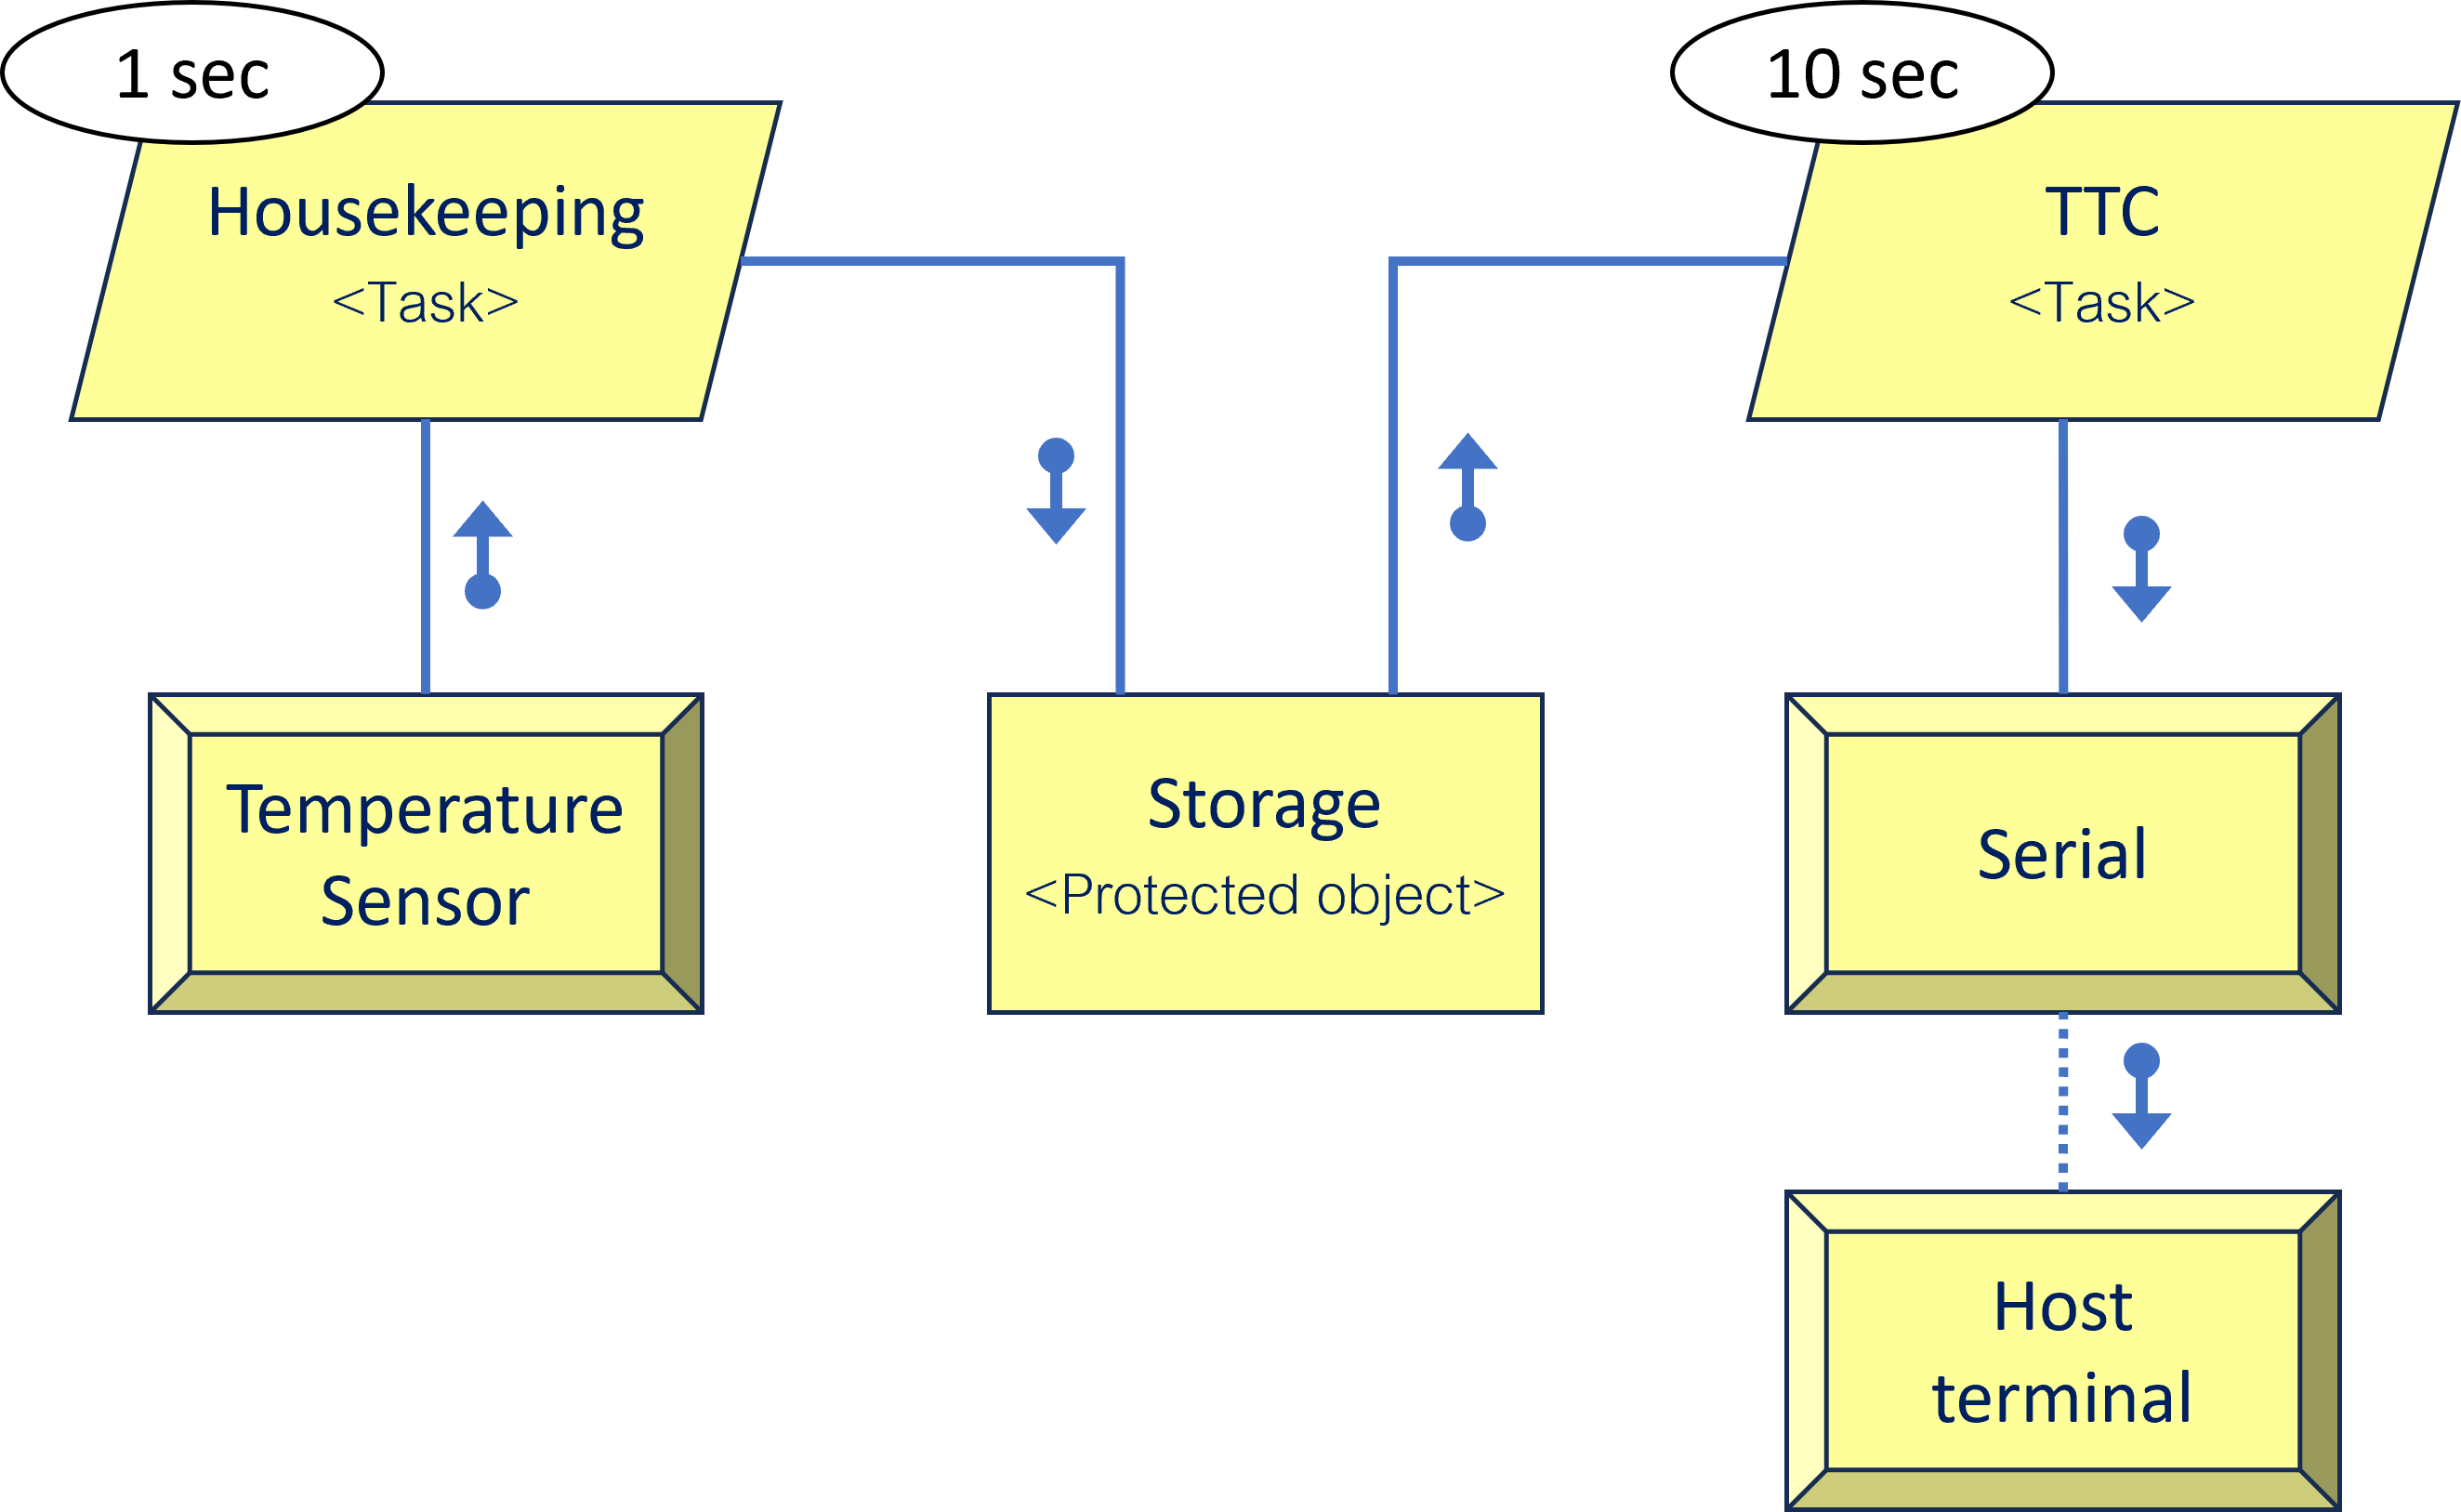
\includegraphics[width=0.8\textwidth,keepaspectratio]{obsw-v2.png}}
	\caption{Software architecture of the OBSW.}
	\label{fig:obdh}
\end{figure}

\begin{description}
\item[Telemetry and Telecommand (TTC).] This component is in charge of the communications with the ground station. The ground station is simulated by the Host terminal. the \texttt{TTC} must be activated cyclically with a 10 second period.

\item[Serial.] This component provides a high-level interface to a text console
where the measured temperature values can be transmitted.

\item[Housekeeping.] Main component,
which performs the basic functionality of the system.
It reads a temperature value and stores it in the \texttt{Storage} component.
It must be activated cyclically with a 1 second period.

\item[Sensor.] This component provides a high-level interface to the temperature sensor and deals with all the details of reading the ADC to which the sensor is connected.

\item[Storage.] This component is a data object storing one temperature value, which is written by \texttt{Housekeeping} and read by \texttt{TTC}. As it is accessed concurrently by two tasks, it must be a protected object guarantying the mutual exclusion.

\end{description}

Since the OBC board does not have a text output device,
temperature values are sent by a serial line to the ground station.
In this way, the radio link between
the satellite and the ground station is
simulated by the \texttt{Serial} and \texttt{Host Terminal} connection (dashed line).

\section{Serial line connections}

This scheme makes use of the USB/UART interface cable provided to the students. The USB/ UART cable has a TTL connector that must be connected to the STM32f4 board pins that convey the serial line (UART) signals (figure~\ref{fig:cable}).

\begin{figure}[h]
    \centering{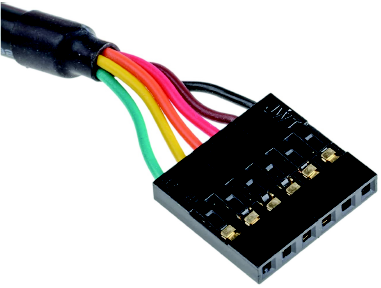
\includegraphics[width=0.3\textwidth,keepaspectratio]{connector.png}}
    \caption{UART cable connector.}
    \label{fig:cable}
\end{figure}

The connections to be made are summarized in the following table (see figure~\ref{fig:board} for the location of the pins on the board):

\begin{table}[htb]
\begin{center}
\begin{tabular}{ll} \hline
Connector pin & Board pin \\ \hline
1 (black) & GND \\
4 (orange) & PB7 \\
5 (yellow) & PB6 \\ \hline
\end{tabular}
\caption{Serial line connections on board.}
\label{tb:connections}
\end{center}
\end{table}

The other end of the interface cable has a USB-A connector
that must be plugged to a USB port on the host computer.
The values sent to the host computer are displayed using a terminal application
that can handle a USB serial port.
The host terminal application should be set to taking the USB serial port as input with
a transmission rate of 115200 bps and
a configuration of 8N1 (8 data bits, no bit parity, 1 bit for stop).

\section{Host terminal application}\label{sc:term}
\subsection{Windows}

The recommended application to display messages received on the USB serial port is PuTTY. You can download an installation package from \url{https://www.putty.org}.

In order to configure the application, you need first to identify the COM port corresponding to the USB serial line. Open the Device Manager and look at the USB Serial Port entry. The COM port is displayed next to it (e.g. COM4 in figure~\ref{fig:com}).

\begin{figure}[hbtp!]
            \centering{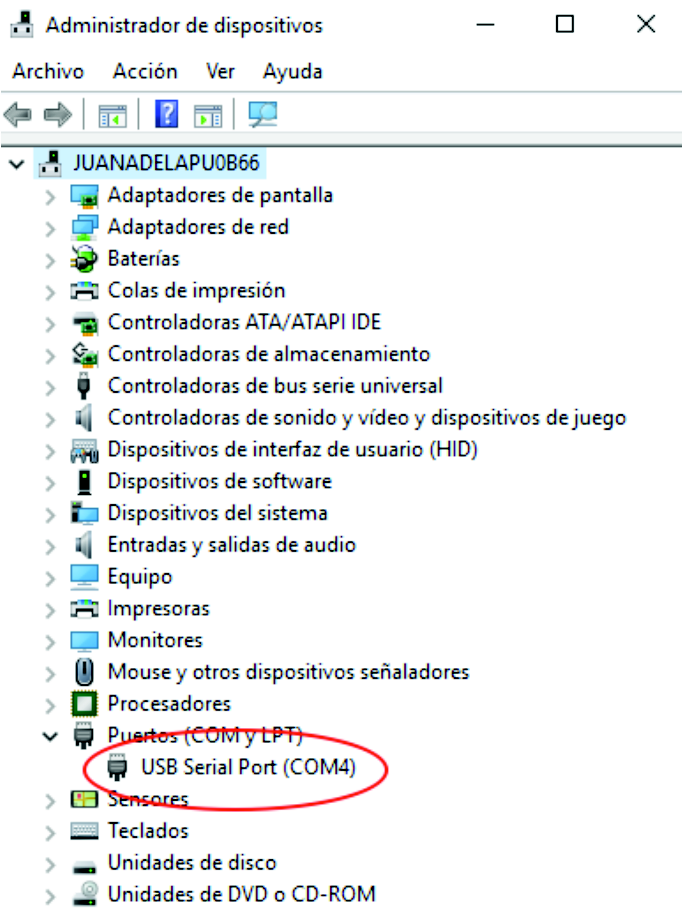
\includegraphics[width=0.6\textwidth,keepaspectratio]{com.png}}
            \caption{Identification of usb serial port.}
            \label{fig:com}
\end{figure}

Now, to set up PuTTY, open the application and set the configuration parameters as shown in figure~\ref{fig:cable}.

\begin{figure}[hbtp!]
            \centering{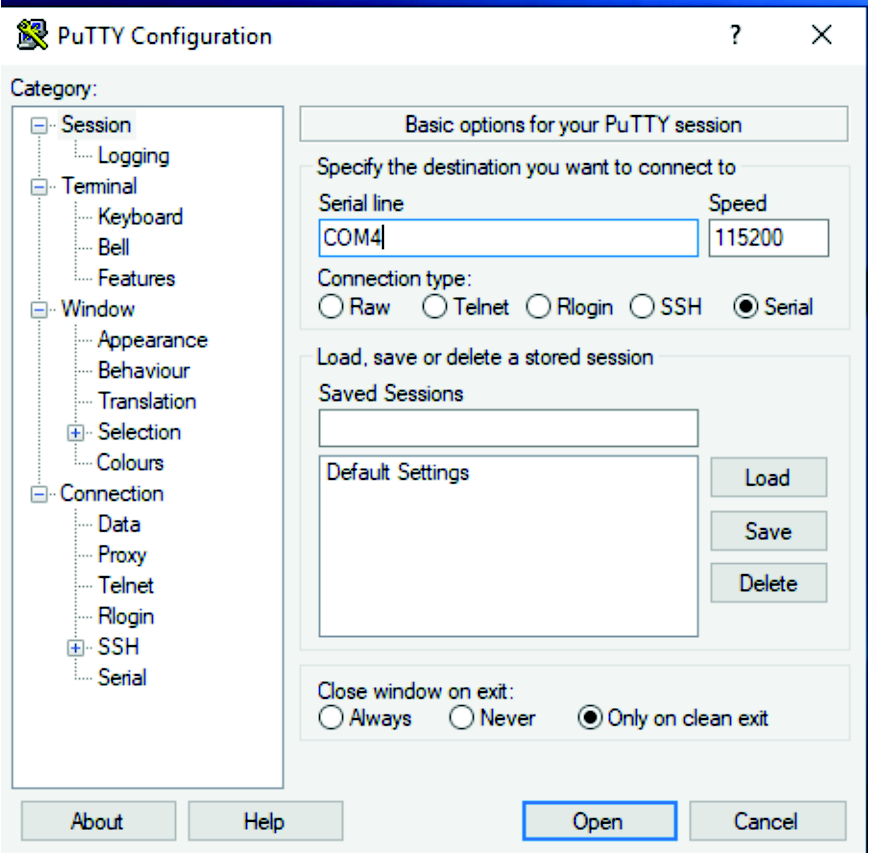
\includegraphics[width=0.6\textwidth,keepaspectratio]{putty.png}}
            \caption{PuTTY configuration.}
            \label{fig:putty}
\end{figure}

\subsection{MacOS}
The recommended application is screen, which is already installed in MacOS.
First you have to identify the USB serial port. Open a terminal window and type

\begin{BVerbatim}
	$ ls /dev | grep -i usb
\end{BVerbatim}

You will get a list of devices like the following:

\begin{BVerbatim}
	cu.usbserial-FTA5I24G
	tty.usbserial-FTA5I24G
\end{BVerbatim}

As you can see, there are two devices for each serial line. You can use any of them, but for reasons not to be discussed here it is better, in general, to use the one starting with cu.

To use the screen application enter the following command:

\begin{BVerbatim}
	$ screen /dev/cu.usbserial-XXXX 115200
\end{BVerbatim}
	
where \texttt{/dev/cu.usbserial-XXXX} is the name of your device.

To exit the application, type CTRL-A and then CTRL-K.

\subsection{GNU Linux}

The recommended application is screen,4 which can be installed in Ubuntu Linux with:

\begin{BVerbatim}
	$ sudo apt install screen
\end{BVerbatim}

In order to identify the USB serial port, type the following command on a terminal:

\begin{BVerbatim}
	$ ls /dev | grep -i usb
\end{BVerbatim}

You will get a result like the following:

\begin{BVerbatim}
	ttyUSB0
\end{BVerbatim}

To use the screen application enter the following command:

\begin{BVerbatim}
	$ screen /dev/ttyUSB0 115200
\end{BVerbatim}

To exit the application, type CTRL-A and then SHIFT-K.

\section{Download the code and study the implementation}

The implementation code, as initially provided to the students, can be downloaded from

\begin{center}
	\begin{tcolorbox}[width=0.6\textwidth,
		boxsep=0pt,
		left=0pt,
		right=0pt,
		top=5pt,
		]
		\centering
		\color{blue}{\url{https://github.com/STR-UPM/SEU-OBDH-Lab}}
	\end{tcolorbox}
\end{center}
 
You can clone the repository or download it as a zip archive.
The code for this assignment is located in the \textcolor{mPurple}{\texttt{lab-3}} folder.

The software components presented in the software architecture section
(figure~\ref{fig:obdh})
are implemented in Ada as packages.
Specifically, the \texttt{Housekeeping} package is the root element of the housekeeping
component.
Its specification consists of one procedure called \texttt{Initialize}
that starts the operation of the component.
The \texttt{Housekeeping} has four subpackages:

\begin{description}
\item[Housekeeping] is the root package of the subsystem and contains a concurrent task, Housekeeping\_Task that stores Data in Storage and toggles the blue LED every second.

\item[Housekeeping.Data] contains the definitions of the data types used in the subsystem. The data type \texttt{Analog\_Data} is used to read the ADC, which are integers in the range 0 to 4095 ($2^{12}-1$) as directly provided by the 12-bit ADC.
The data type \texttt{State} is a record that contains the ADC reading and the corresponding timestamp.

These ADC values have to be converted to engineering units. i.e. degrees Celsius, by following the specification of the temperature sensor (se appendix~\ref{ap:sensor}).
Unless the sensors readings must be used to contorl the satellite,
raw readings are usually sent to ground station
that is in charge of converting them to engineering units.
This way, the OBSW is kept as simple as possible.

\item[Housekeeping.Sensor]  is a low level component
that contains the implementation details of the temperature sensor.
Its specification includes the \texttt{Initialize} and \texttt{Get} procedures.
This package uses the Ada Drivers Library to interact with the OBC board hardware.

\item[Housekeeping.Images] includes functions which are used to convert the temperature and timestamp values to Strings. These functions are called \texttt{Image} per the Ada language conventions,
similar to \texttt{printf} in $\ast$nix environments.
\end{description}

The \textbf{TTC} package is the root of the telecommunications system, which in this version is greatly simplified with respect to a real application.
It contains a concurrent task,
\texttt{HK\_Task},
which periodically obtains the sensor measurements located in the \texttt{Storage} and sends them to the ground station by using \texttt{Serial}.
This activity is performed with a period of ten seconds.
The task also toggles the orange LED for a visual inspection.

The \textbf{Storage} package implements the communication between the \texttt{Housekeeping} and \texttt{TTC} subsystems. 
Since this object is shared by two concurrent tasks, it is implemented as a \textit{protected object},
so that its operations are executed in mutual exclusion.
There is also \textit{conditional synchronization}:
the \texttt{TTC} task must wait until there is a fresh value in the store.
However, \texttt{Housekeeping} should not wait if the previous values put into Storage have not been consumed, in order not to delay the housekeeping function.
In this case, the stored value is overwritten. Notice that this differs from the classical specification of a bounded buffer.

The \textbf{Serial} component is implemented by the \texttt{Serial.IO} package and other packages in the \textcolor{mPurple}{\texttt{serial\_ports}} folder.
These packages have been adapted from the examples in the Ada Drivers Library.
The blocking kind of serial port was chosen for this project.
This means that the task calling the \texttt{Put} operation (\texttt{TM\_Task}) waits on a busy loop (aka. active wait) until the operation is complete.

The main procedure is \textbf{OBSW}.
It calls \texttt{Housekeeping.Initialize},
which initializes the sensor so that \texttt{Housekeeping\_Task} can proceed.
Additionally, the green LED is toggled on and off to provide a visual check that the program is running.

Notice that \texttt{Run}, and hence \texttt{Initialize} and \texttt{OBSW}, never return. Therefore the program executes indefinitely, as is common in embedded systems.
Also note that the Main task runs at the lowest priority level
(\textcolor{mGreen}{\texttt{Main.ads:23:}} \textcolor{blue}{\texttt{with Priority => System.Priority'First}}) to let other components run when they are active.

\section{Compile and run}\label{sec:ass-2:compile-run}

Open GPS and do the following:
\begin{enumerate}
\item Select Open project on the welcome window. Navigate to the \textcolor{mPurple}{\texttt{SEU-OBDH-Lab/lab-3}} directory and open the \texttt{realtime\_housekeeping.gpr} project file.
\item Build the executable and load it into the board by clicking on the \hbox{
\includegraphics[width=1.5em]{buildandload.png}} symbol in the tool bar (or select Build $\rightarrow$ Bareboard $\rightarrow$ Flash to board on the top menu).

The program will be compiled, and the executable will be loaded into the board flash memory. After that, the program starts to run on the board (check the blinking LEDs).
\item Connect the serial cable to a USB port on the host computer, if not already done.
\item Identify the serial port name on the host computer and launch the remote terminal application as explained in section~\ref{sc:term}. The sensor measured values together with their respective timestamps will start being displayed on the host application (figure~\ref{fig:output}).
\end{enumerate}

\begin{figure}[h]
            \centering{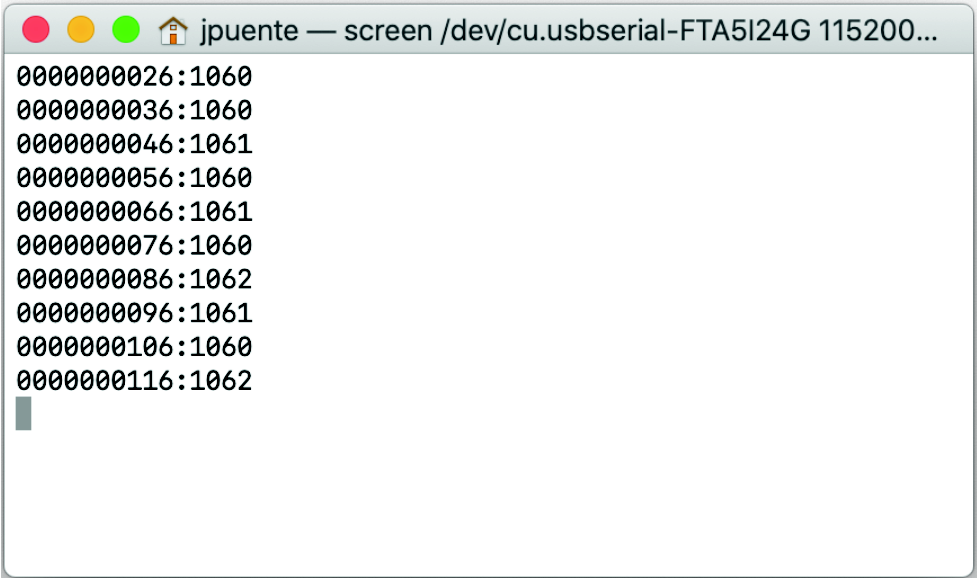
\includegraphics[width=0.6\textwidth,keepaspectratio]{output.png}}
            \caption{Sample output on host terminal.}
            \label{fig:output}
\end{figure}

\section{Make changes to the program}

It is advised that you may make changes
to the provided program in order to make sure
that you understand the project implementation,
and the mapping from the architecture to source code.

\textcolor{mRedBrown}{\textit{The proposed change is to}}: Include the conversion to Celsius in the \texttt{TTC.Send} procedure.
The temperature transfer function is implemented by \texttt{HK\_data-converter}
which can be found in utilities.

\section{Perform a temporal analysis of the system}\label{sc:ta}

Real-time systems need to fulfill temporal requirements,
like activation patterns (cyclic/periodic or sporadic),
the activation periods of the tasks,
or guaranteeing the \textit{schedulability} of the system.
The latter ensures the \textit{temporal behaviour} of the system,
which means that \textit{all tasks
execute within their deadlines}.
This is assured analytically by conducting a \textbf{Response-Time Analysis (RTA)}.
To perform the RTA, you will need to measure the execution time of the task bodies and the protected procedure bodies.
A simple loop technique using the standard real-time clock will be enough for this assignment.

An execution time measurement tool is available in the \textcolor{mPurple}{\texttt{lab-3}} directory.
In order to use it, perform the following steps:

\begin{enumerate}
\item Open GPS and select Open project on the welcome window. Navigate to the \textcolor{mPurple}{\texttt{lab-3}}
directory and open the \texttt{wcet\_meter.gpr} project file.

\item Build the executable and load into the board in the same way as for the \texttt{realtime\_housekeeping.gpr} project, see section~\ref{sec:ass-2:compile-run}.

\item Make sure that the serial cable is still connected to the board and the USB port in the host
computer. If the remote terminal application is not open, open it.
\end{enumerate}

A measurement test is executed on the board, and repeated every 60 s. The output of the test is shown on the host terminal application (figure~\ref{fig:wcet}). The output shows the execution times for the bodies of the Housekeeping (HK) and TTC (TC) tasks, as well as the bodies of the protected operations of the Storage object (ST). Notice that a new entry, \texttt{Get\_Immediate},
has been added for the latter in order \textit{to avoid the measuring task to get blocked}.
The new entry is exactly the same as \texttt{Get} but has a True barrier so that it is always open.

\begin{figure}[h]
    \centering{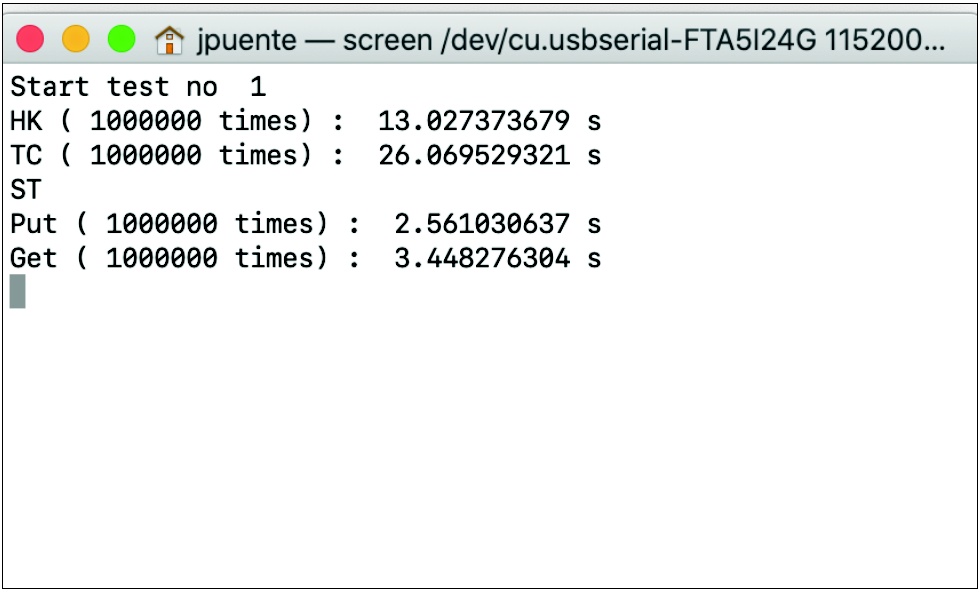
\includegraphics[width=0.6\textwidth,keepaspectratio]{wcet.png}}
    \caption{Output of wcet measurement tool.}
    \label{fig:wcet}
\end{figure}

In the example shown on figure~\ref{fig:wcet}, the HK execution time has been measured $10^{6}$ times, with a total measurement time of 13.02 s. Therefore, the value to be taken for the response time analysis is $13.02\cdot10^{-6}~s = 13.02~\mu${s}, and the same for the other tasks. Take into account that the values measured on your board will probably be slightly different from the above shown.

Once you have an estimate of worst case execution times, apply the RTA equations for computing the worst-case response time and check if all the deadlines are met. The setup for the calculations is shown on table~\ref{tb:wcet}
containing the period (T), execution time (C),
blocking time (B), deadline (D),
response time (R), priority (P),
and accesses to protected object of each task.

\textcolor{mRedBrown}{\textbf{Important}}: The temporal analysis (RTA) will be explained later in the course. Therefore, execution times should be stored for later. 

\begingroup
\setlength{\tabcolsep}{8pt} % Default value: 6pt
\renewcommand{\arraystretch}{1.2} % Default value: 1

\begin{table}[htb]
\begin{center}
	
	\small % Font size
	
	\begin{tabular}{|r r r r r r r r r|} \hline
	\textbf{Task} & T & C & B & D & R & P & Storage & Operation\\ \hline
	
	\textbf{Housekeeping} & 1.0 & $13\cdot10^{-6}$ & \textcolor{mRedBrown}{\textbf{?}} & 1.0 & \textcolor{mRedBrown}{\textbf{?}} & 20 & $3\cdot10^{-6}$ & CPut \\
	
	\textbf{TTC} & 10.0 & $26\cdot10^{-6}$ & \textcolor{mRedBrown}{\textbf{?}} & 2.0 & \textcolor{mRedBrown}{\textbf{?}} & 10 & $4\cdot10^{-6}$ & CGet \\ \hline
	
	& & & & & & CP & \multicolumn{2}{|c|}{\textcolor{mRedBrown}{\textbf{?}}} \\ \hline
	\end{tabular}
	\caption{Data arrangement for RTA of the housekeeping system. Time units in seconds.}
	\label{tb:wcet}
\end{center}
\end{table}

\endgroup


	\chapter{OBDH with ACS}\label{ch:obdh-acs}

The aim of this assignment is to validate the Attitude Control System (ACS)
with the Processor In the Loop (PIL) technique.
PIL consists on simulation from the external environment
through mathematical models (in Simulink)
that are directly connected to the onboard computer.
This way, we can analyze the system's behaviour
based on simulated readings and actuations performed by the OBSW.

The reduced version of an OBSW
is used with the ACS of the UPMSat-2 satellite.
The ACS uses magnetic sensors (magnetometers) and actuators (magnetorquers).
This system conforms to a magnetic attitude control (figure~\ref{fig:acs}).

\begin{figure}[hbtp!]
	\centering{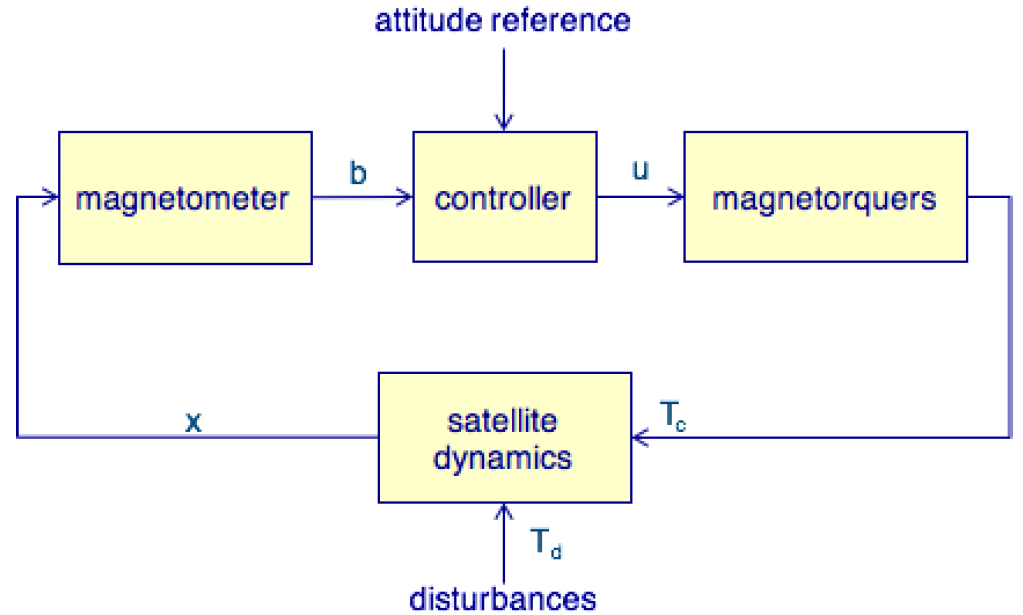
\includegraphics[width=.6\textwidth,keepaspectratio]{acs.png}}
	\caption{Magnetic attitude control system.}
	\label{fig:acs}
\end{figure}

\textbf{Magnetometers} are magnetic sensors
that provide a measurement of the strength
and direction of the magnetic field, i.e. the magnetic field vector,
at a given point.
\textbf{Magnetorquers} are magnetic coil which produce a magnetic moment that interacts with the Earth's field,
thus enabling the attitude of the satellite to be changed.

% -- MIL ------------------------------------------------------------------------

\section{Model In the Loop (MIL) validation}

Software validation usually includes testing the system under real operating conditions.
However, for obvious reasons, on-board space software as well as many other embedded systems cannot be tested in this way.
Simulation models are commonly used in these cases.

The first validation phase uses a model of the ACS,
together with models of the space environment and the spacecraft dynamics,
to assess the validity of the control law and the design parameters (figure~\ref{fig:acs-hl}).
This is usually carried out by a control engineer using a simulation tool.
Simulink is commonly used for ACS development.

\begin{figure}[hbtp!]
    \centering{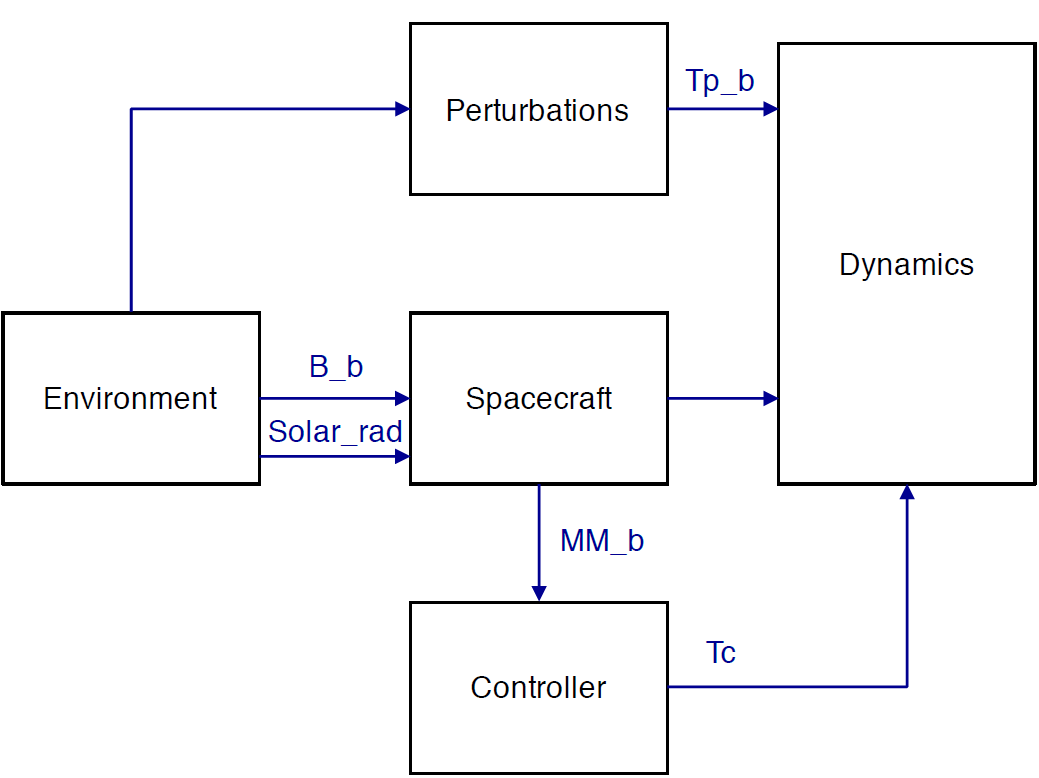
\includegraphics[width=0.6\textwidth,keepaspectratio]{acs-hl.png}}
    \caption{UPMSat-2 ACS high level model view.}
    \label{fig:acs-hl}
\end{figure}

The ACS Simulink model can be simulated by running MATLAB from the
\textcolor{mPurple}{\texttt{lab-4/acs}}
directory and opening \texttt{ACS.slx}.
Three new windows will pop-up: the Simulink window with the ACS model
and two scope windows that show the angular velocity of the satellite in body reference and the actuation over its three magnetorquers.

The Simulink window (figure~\ref{fig:acs-simulink}) shows the high level blocks: the satellite's model is located in the middle (turquoise block),
its dynamics and the models of the Earth's field and Sun with the perturbations.

\begin{figure}[hbtp!]
    \centering{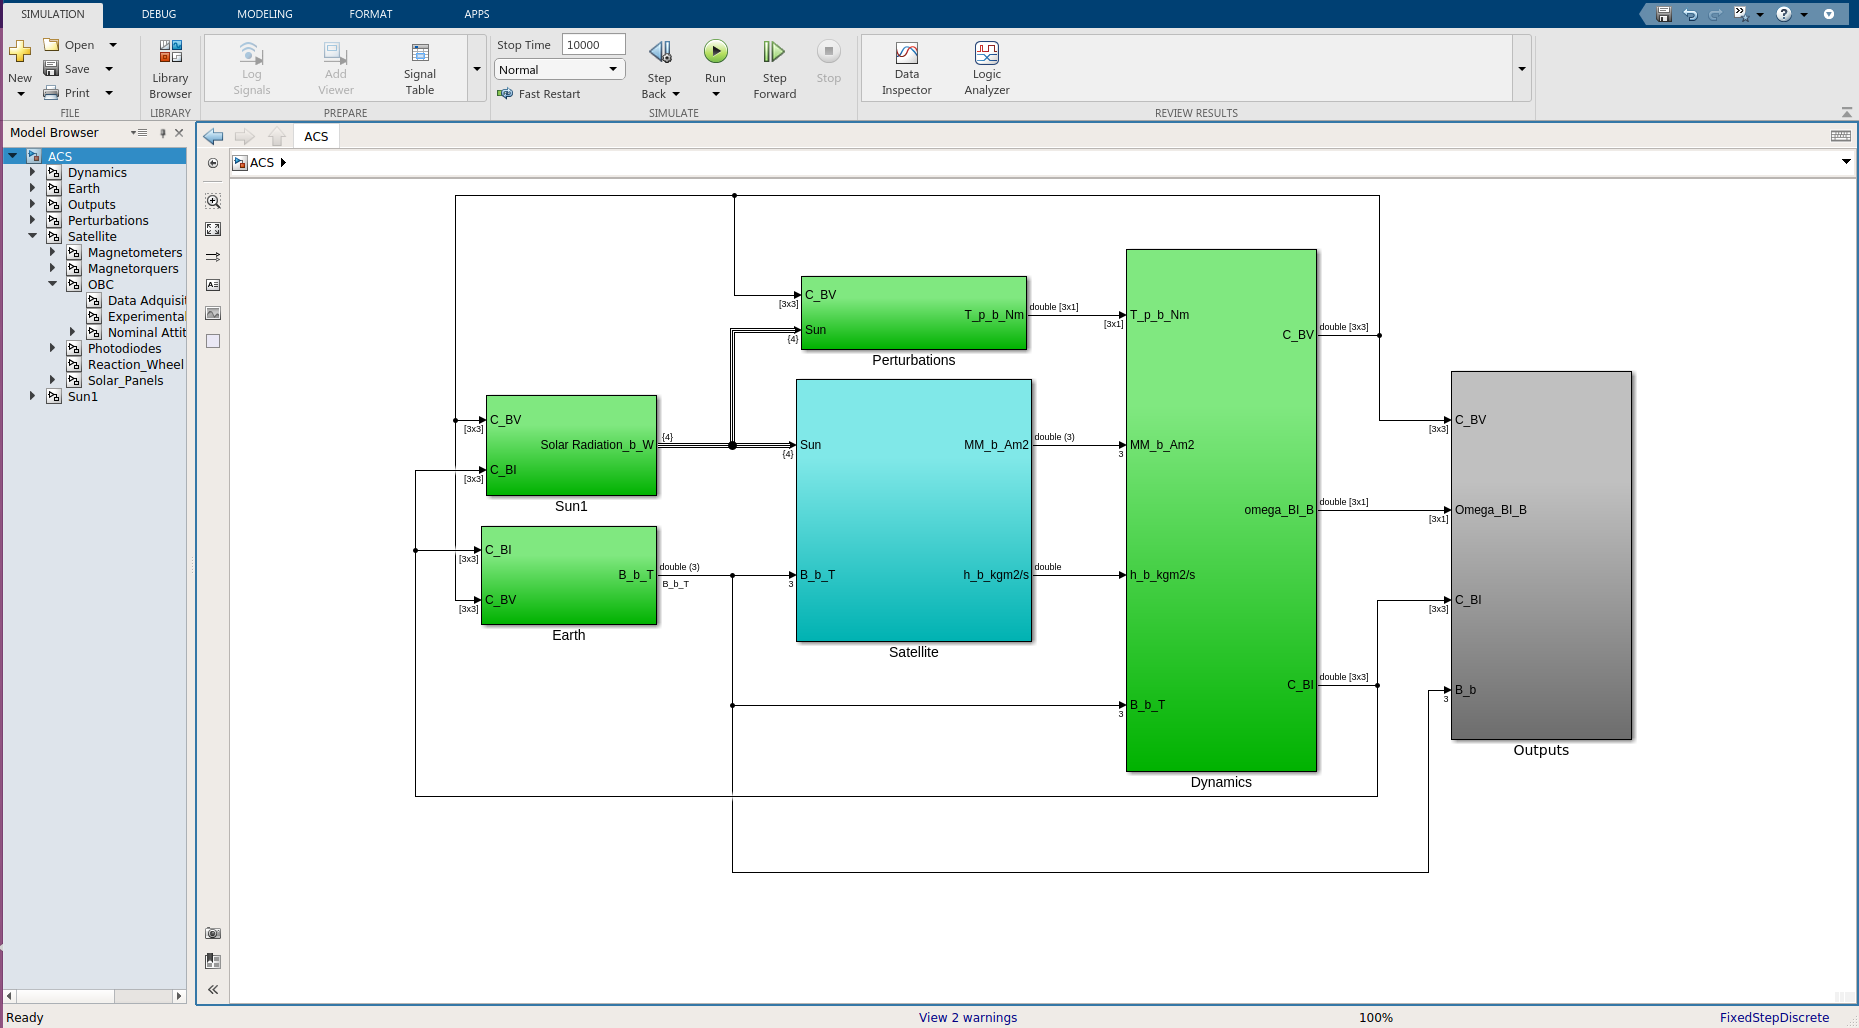
\includegraphics[width=\textwidth,keepaspectratio]{acs-simulink.png}}
    \caption{UPMSat-2 Simulink model.}
    \label{fig:acs-simulink}
\end{figure}

The nominal attitude control can be visualized
by selecting Nominal Attitude Control in the Model Browser menu
(left part of simulink window) or by clicking on Satellite $\rightarrow$ OBC $\rightarrow$ Nominal Attitude Control blocks. The Nominal attitude control has three blocks (figure~\ref{fig:nac}):
\begin{description}
\item[Sensor] samples the analog inputs of the magnetometers. The inputs are converted to engineering units using calibration data.
\item[Control] implements the attitude control law that computes the control action to be output to the magnetorquers.
\item[Actuator] activates the magnetorquers according to the computed control action.
\end{description}

\begin{figure}[H]
            \centering{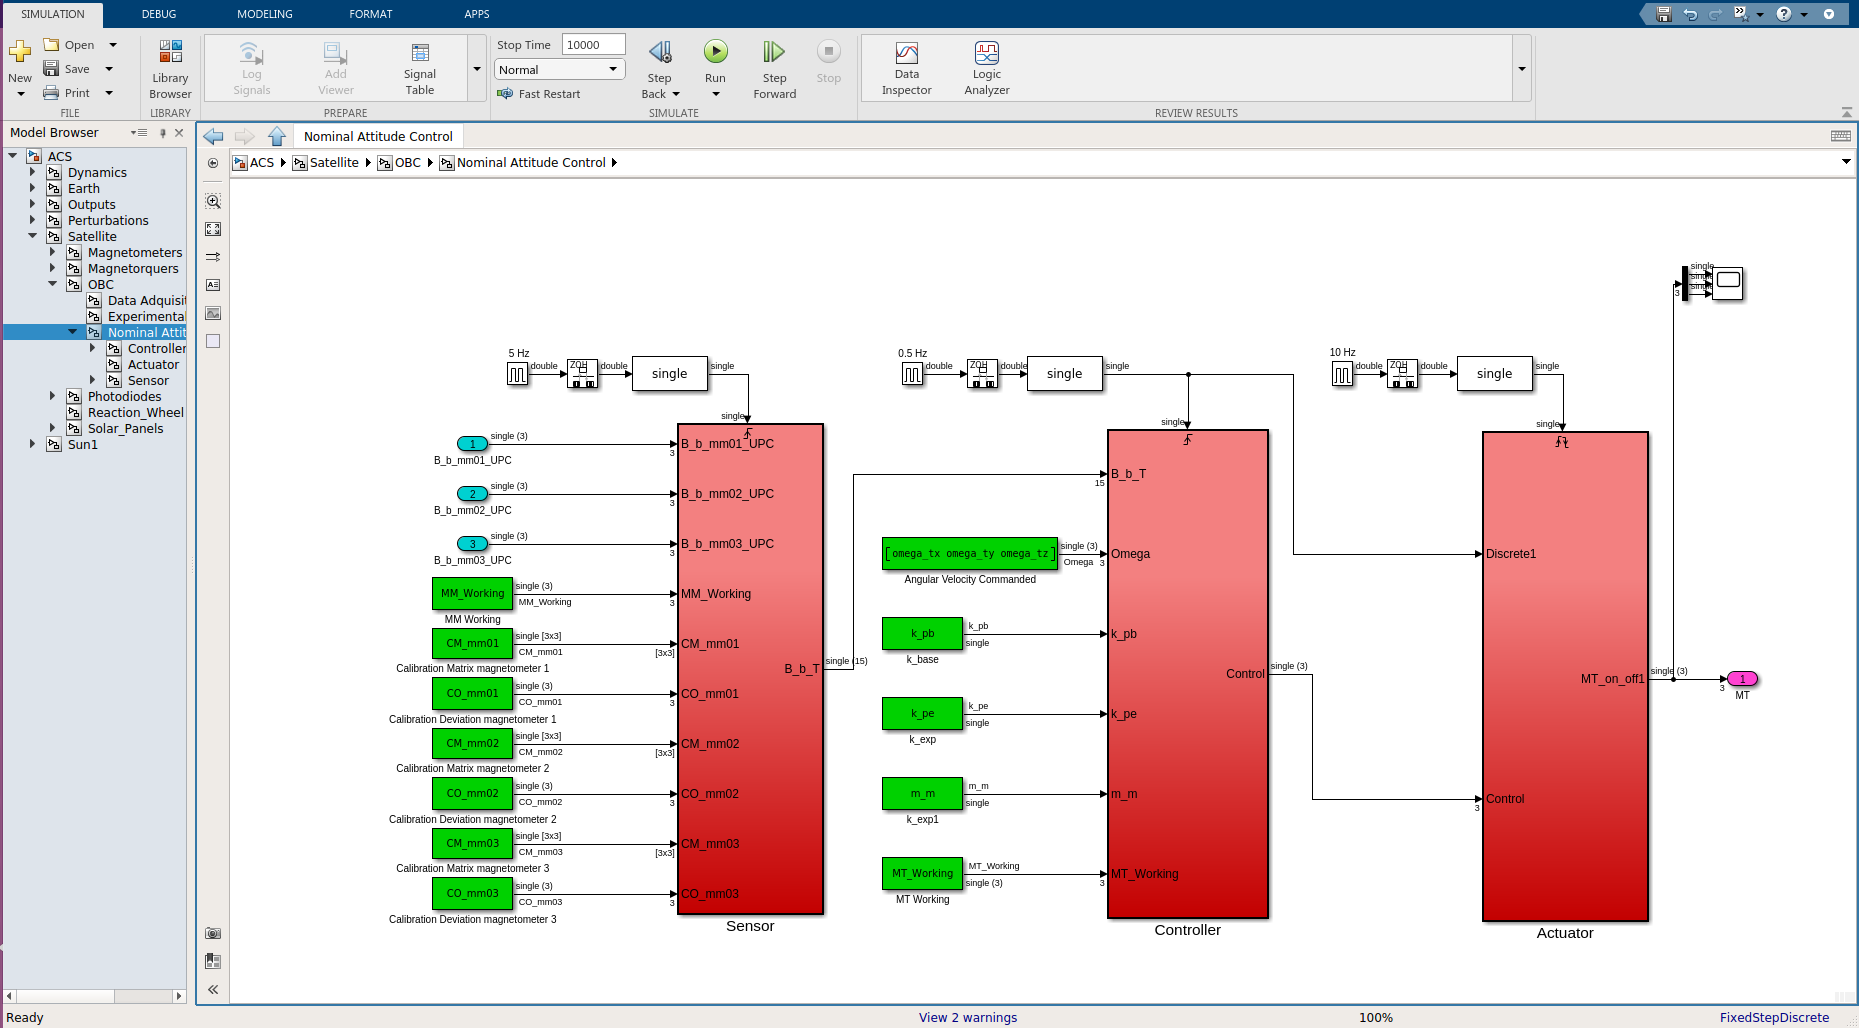
\includegraphics[width=\textwidth,keepaspectratio]{nac.png}}
            \caption{Nominal attitude control.}
            \label{fig:nac}
\end{figure}

To simulate the model an verify its behaviour,
click on Run bottom.
The evolution of the angular velocity of the satellite
and the actuation over the three magnetorquers will be shown in the corresponding scope windows.
The commanded angular velocity set-point is [0, 0, 0.1] rad/s
and the result of the simulation (figure~\ref{fig:scope})
shows the evolution from the initial angular velocity ([0.1, -0.1, -0.1] rad/s).

\begin{figure}[h]
    \centering{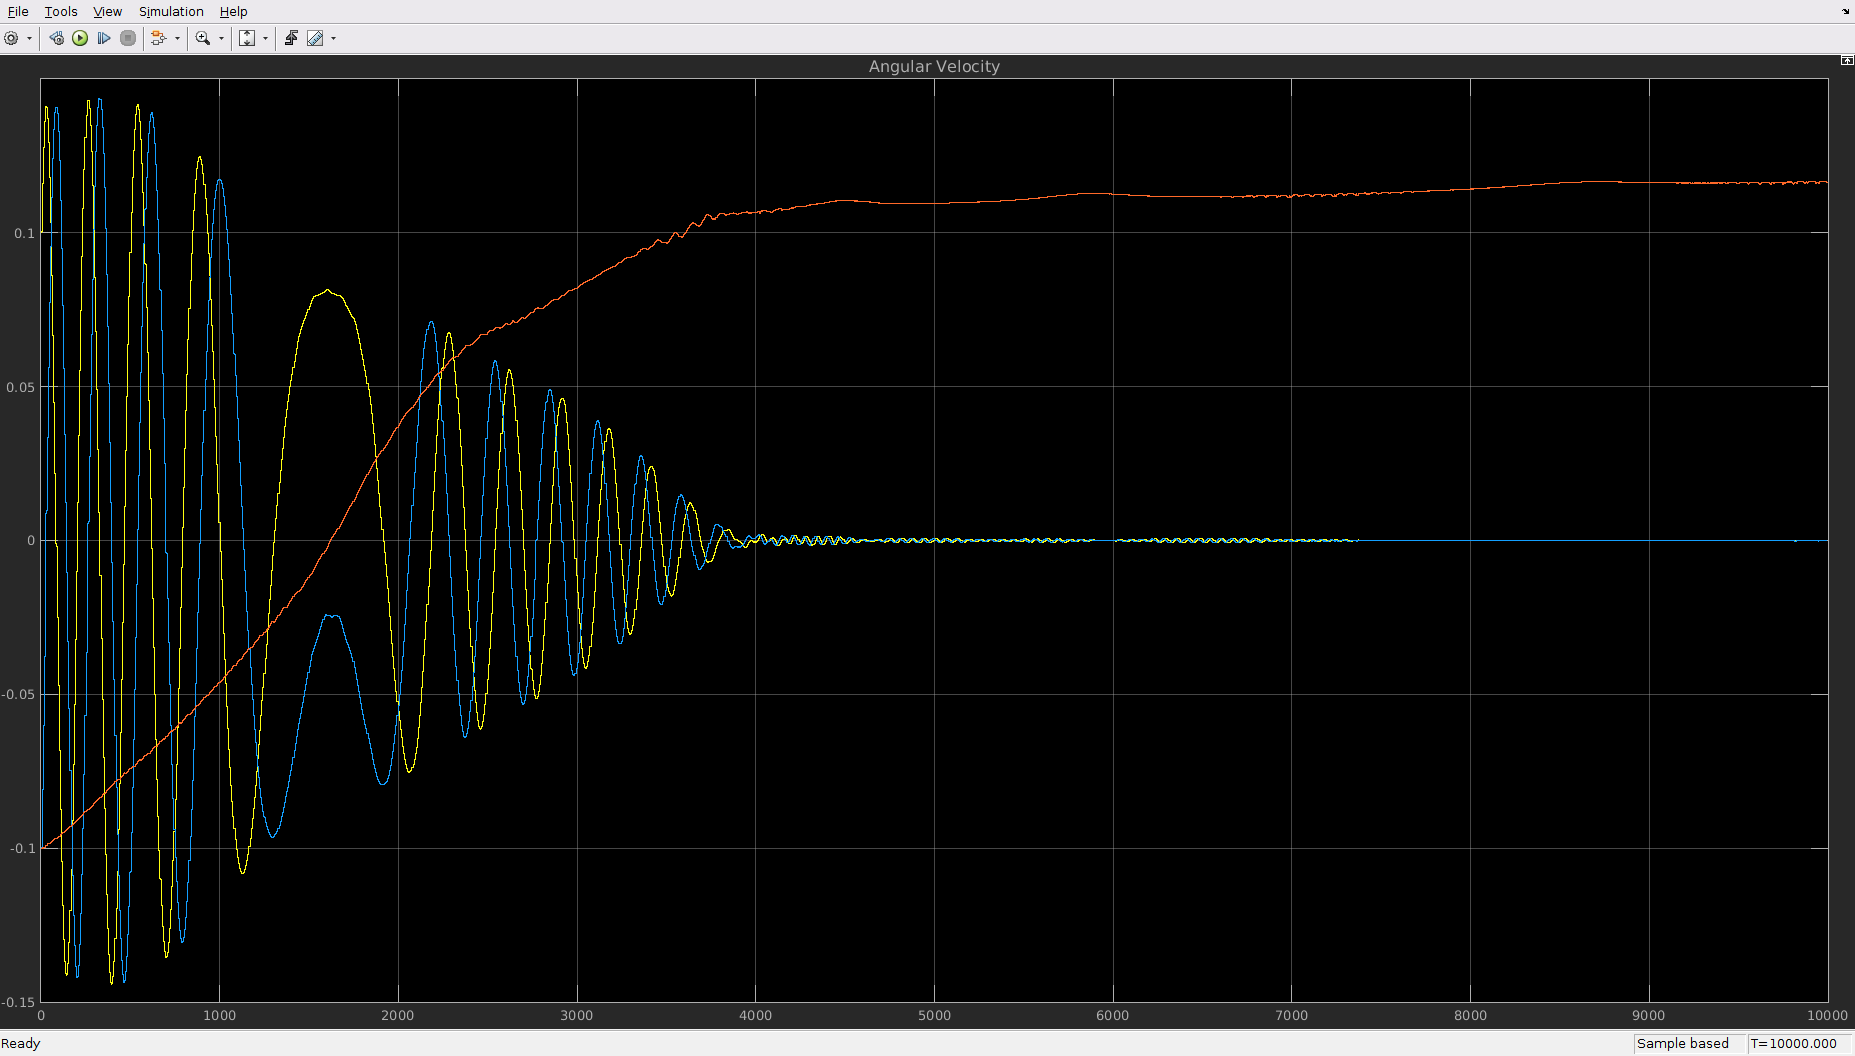
\includegraphics[width=\textwidth,keepaspectratio]{scope.png}}
    \caption{Angular velocity evolution.}
    \label{fig:scope}
\end{figure}

\section{Code generation}

The next step is to execute the ADCS on the board.
In this assignment, only the \texttt{Control} block will be executed on the target board.
The corresponding code can be generated by using the \textbf{Embedded Coder} toolbox but it is needed to isolate \texttt{Control} block from the ACS model.
It can be done by clicking in the Control block,
selecting all the block content (except the trigger block)
and saving it in a new model.

This model named \texttt{control.slx} can be found in \textcolor{mPurple}{\texttt{lab-4/acs}} directory.
Open it with MATLAB and then select APPS in the top menu,
Embedded Coder will appear.
If not, it must be installed by clicking Get Add-Ons and searching it.
The Embedded Coder window (figure~\ref{fig:control}) will appear after clicking on Embedded Coder icon.

\begin{figure}[h]
	\centering{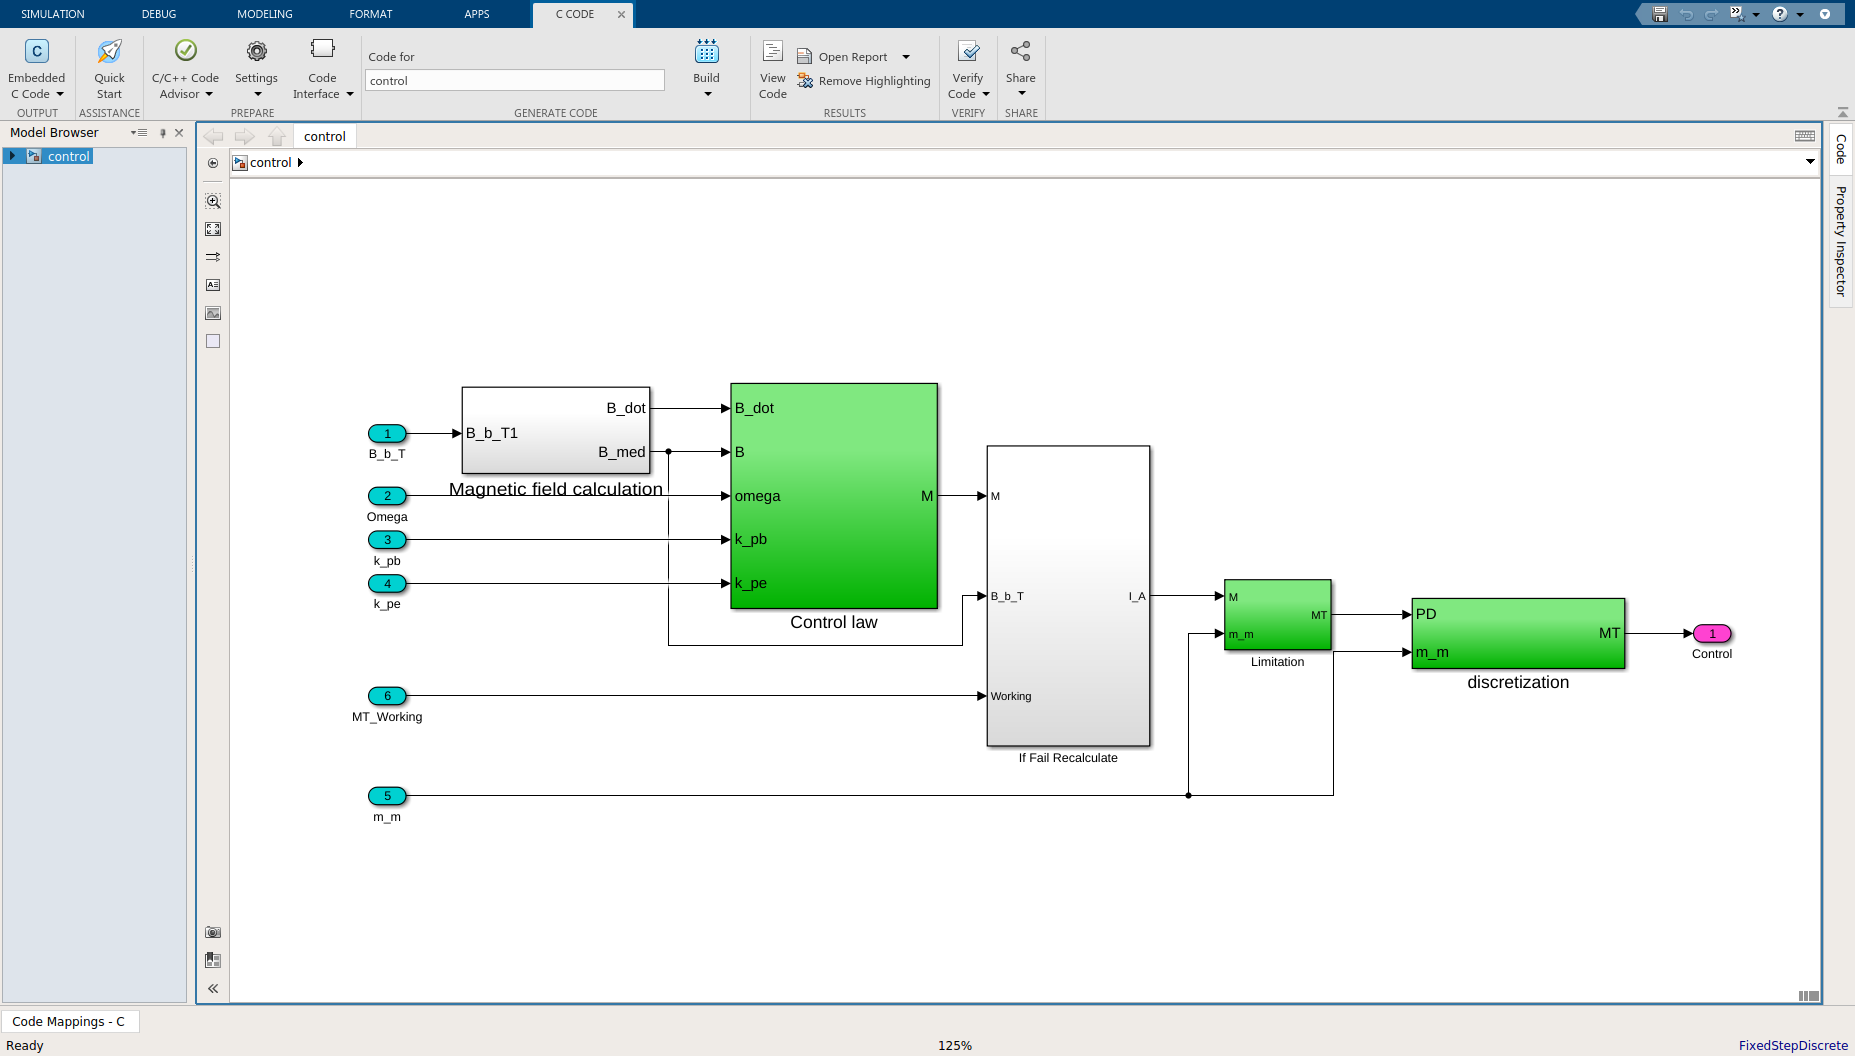
\includegraphics[width=\textwidth,keepaspectratio]{control.png}}
	\caption{Embedded Coder toolbox.}
	\label{fig:control}
\end{figure}

The code generation option as well as characteristics of the target hardware
can be set by clicking on the Settings menu.
The \texttt{control.slx} model has already the proper options,
therefore you can take a look but be carefully and do not modify them.

Now, the code can be generated by clicking on the Build menu.
Once upon the code is generated,
a code generation report window appears.
It is possible to explore the generated code together with different code metrics.
Click on \texttt{control.h} and look for lines 50-79 (figure~\ref{fig:code}) where the generated code interface is located.

\begin{figure}[hbtp!]
    \centering{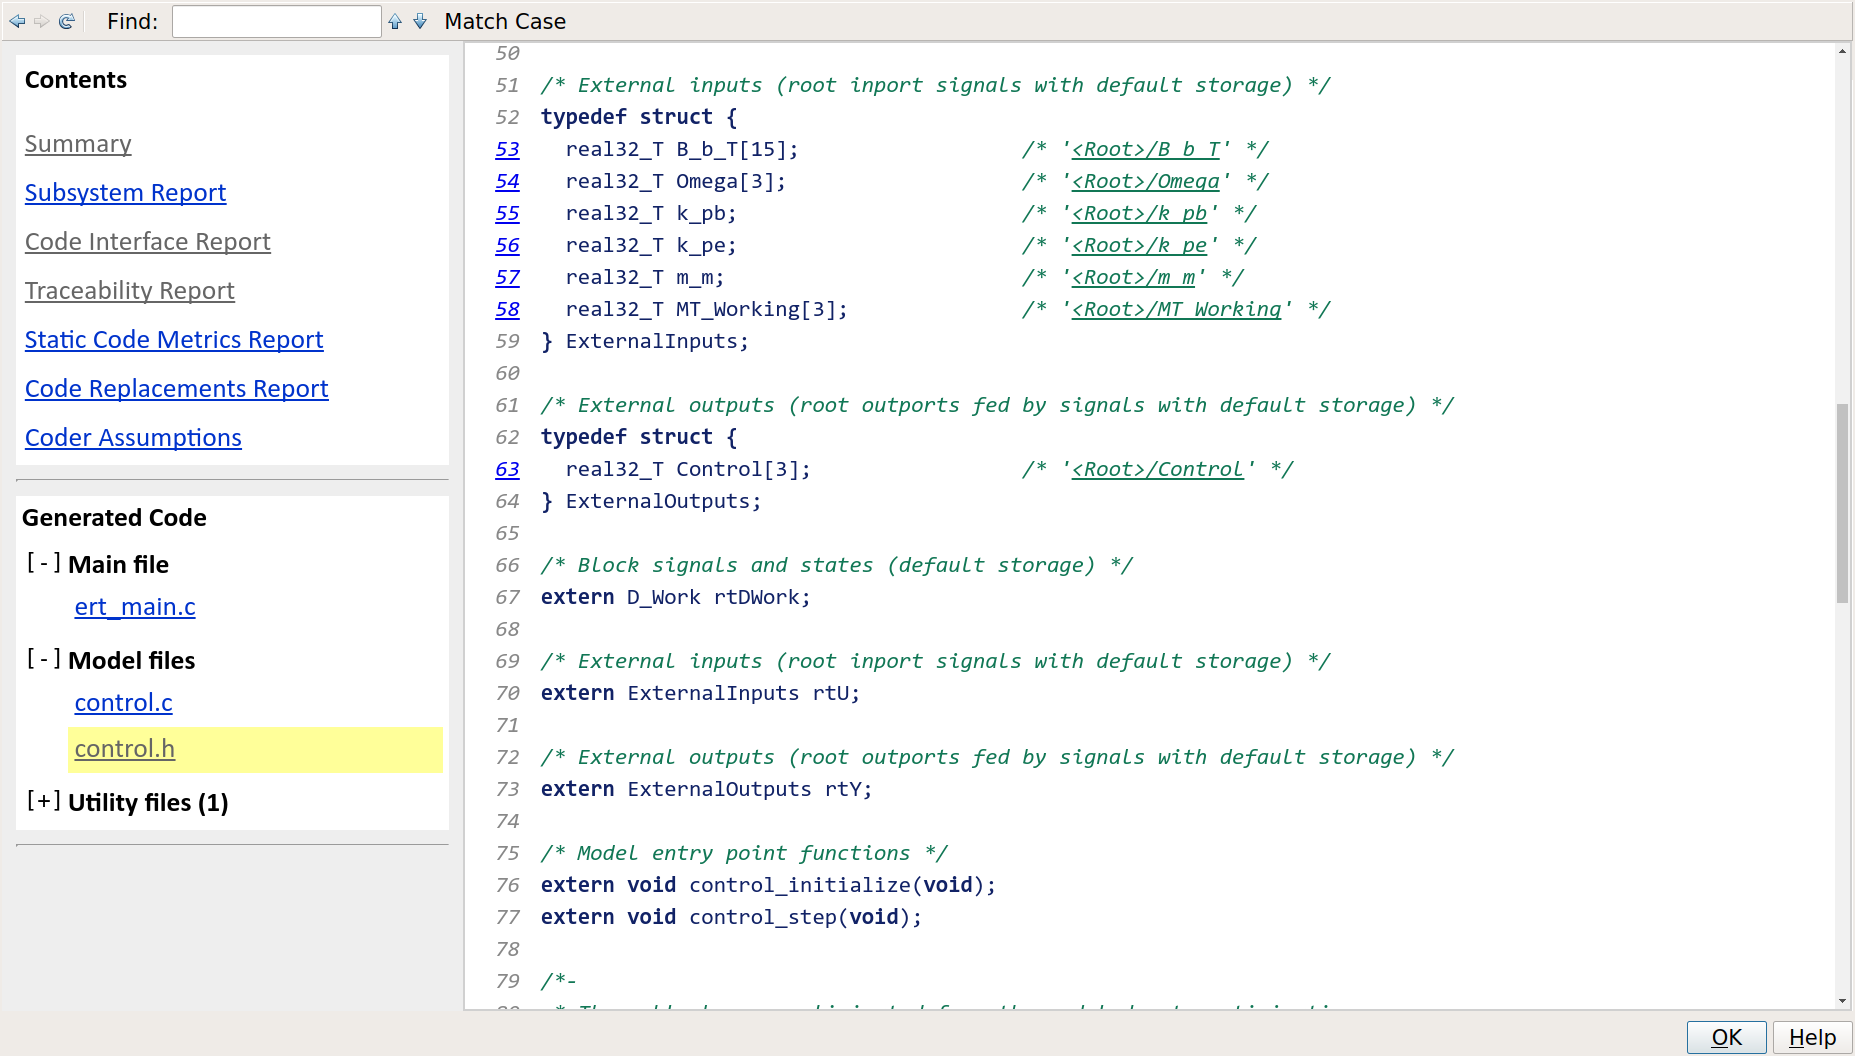
\includegraphics[width=\textwidth,keepaspectratio]{code.png}}
    \caption{Code generation report.}
    \label{fig:code}
\end{figure}

There are two record type definitions (C structs) called \texttt{ExternalInputs} and \texttt{ExternalOutputs}
that are used to interchange data with the blocks
Sensor and Actuator (figure~\ref{fig:nac}).
Data are interchanged with two global variables: \texttt{rtU} and \texttt{rtY}.
Moreover, function \texttt{control\_initialize}
initializes the control code and function \texttt{control\_step}
performs the control algorithm.
The generated code will be embedded in the OBSW by taking into account this interface.

\section{Software architecture}

The implementation code, as initially provided to the students, can be downloaded from \url{https://github.com/STR-UPM/SEU-OBDH-Lab/ass-3}.

\begin{figure}[H]
            \centering{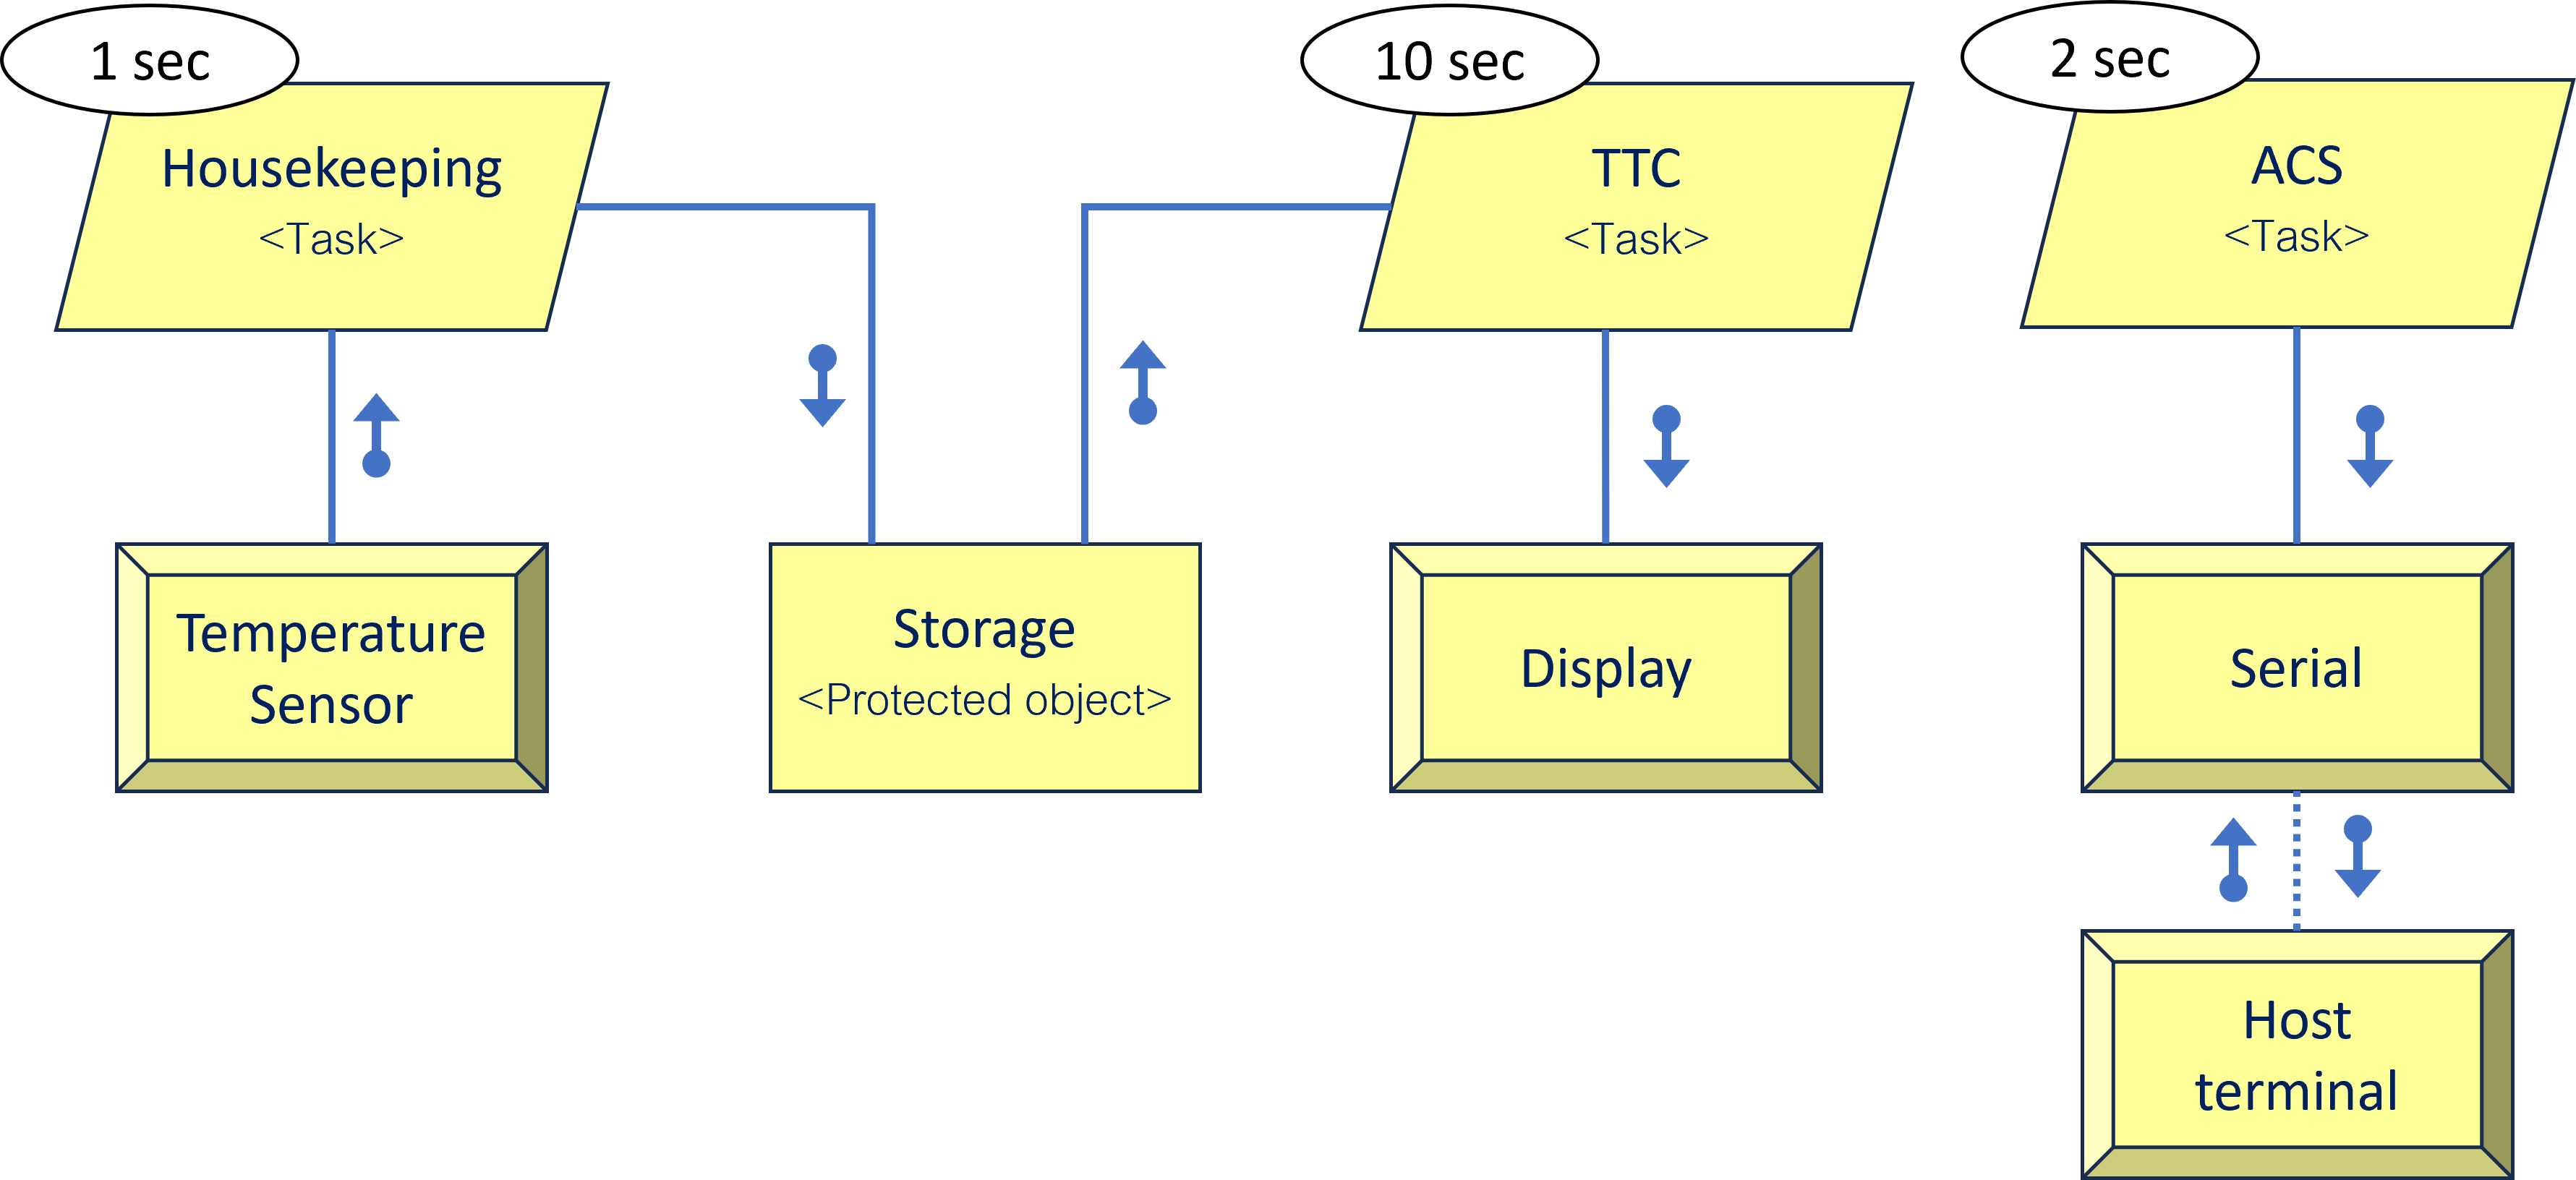
\includegraphics[width=\textwidth,keepaspectratio]{obsw-acs-v2.png}}
            \caption{Software architecture of OBSW with ACS.}
            \label{fig:obdh-acs}
\end{figure}

The software architecture of the OBSW with ACS is depicted in figure~\ref{fig:obdh-acs} and the differences with the previous architecture (figure~\ref{fig:obdh}) are:

The ADCS package is the root element of the ADCS. Its specification consists of one procedure, Initialize, that starts the operation of the component. It has three subpackages:
\begin{description}
\item[ADCS] is the root package of the subsystem and contains a concurrent task, ADCS\_Task that reads the magnetic field vector, calculates the torque vector and sends it to magnetorquers. It also toggles the red LED every two second.
The body of this package uses the generated code by setting the inputs, calling the functions and retrieving the outputs following the interface of figure~\ref{fig:nac}.
\texttt{ADCS\_Task} performs the control algorithm by calling \texttt{control\_step}.
This is shown in figure~\ref{fig:acs-body}.
It uses Export and Import pragmas to interface the generated C code.

\begin{figure}[h]
            \centering{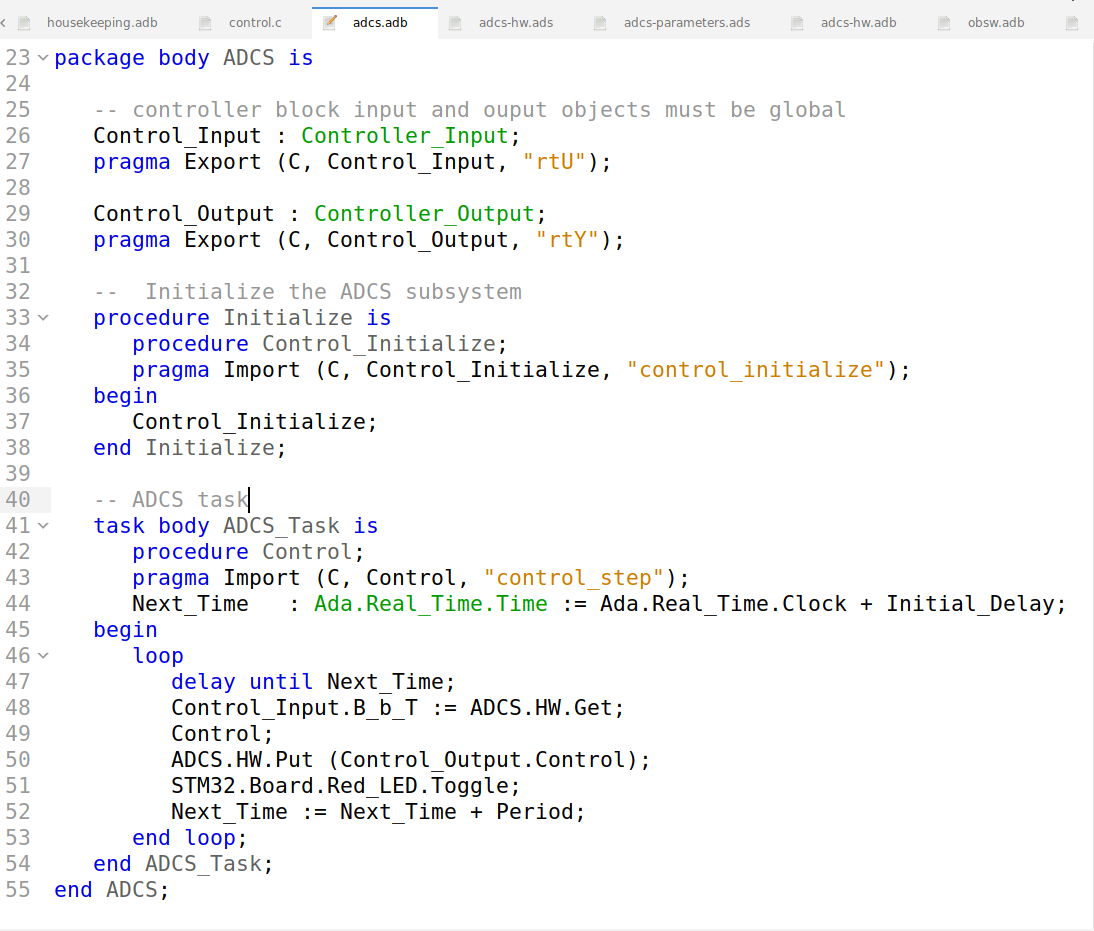
\includegraphics[width=\textwidth,keepaspectratio]{acs-body.png}}
            \caption{Implementation of ACS package.}
            \label{fig:acs-body}
\end{figure}

\item[ADCS.Parameters] contains the definitions of the data types used in the subsystem and parameters that are used to tune the control algorithm. These parameters can be changed by telecommand in the UPMSat-2 OBSW. The data type Controller\_Input is used to read the magnetic field vector in teslas, which are IEEE single precision float numbers. The data type Controller\_Output are used to send the actuation to magnetorquers in newton-meters, which are IEEE single precision float numbers. These data types correspond to the generated C structs ExternalInputs and ExternalOutputs (see figure~\ref{fig:code}), taking advantage of the C and Ada languages interoperability.

\item[ADCS.HW] is in charge of getting the magnetic field vector and putting the
torques. It hides the details of the hardware. Its specification includes the \texttt{Put} and \texttt{Get} subprograms.
This package uses the serial port to interchange magnetic field and torque values with the Software Validation Facility (SVF).
\end{description}

The SVF is an auxiliary computer (the student's PC),
linked to the OBC by a serial line, to run a simulation model of the Earth's magnetic field and satellite dynamics. In this way, engineering values (Nm and T) can be interchanged.

Host computers are also used as SVF by executing a Simulink\texttrademark model of the Earth's magnetic field and satellite dynamics.

In this assignment, the serial line is used to interchange data between ADCS and SVF. Therefore, housekeeping telemetry are send to a text console that is simulated on the host computer, using a mechanism called semihosting. When the target board is connected to the host by means of the ST-LINK USB cable, and the embedded program is run using the debugger in the host, the standard output is re-directed to the debugger console. The GPS environment supports semihosting.

\section{Compile and run with the debugger.}

Open GPS and do the following:
\begin{enumerate}
\item Select Open project on the welcome window. Navigate to the OBSW directory and open the realtime\_housekeeping.gpr project file.
\item Build the executable and load it into the board by clicking on the \hbox{
\includegraphics[width=1.5em]{debug.png}} symbol in the tool bar (or select Build $\rightarrow$ Bareboard $\rightarrow$ Debug on board on the top menu).

The program will be compiled, and the executable will be loaded into the board memory by the debugger. The debugger console (lowest window in GPS) shows the following lines:
\begin{verbatim}
...
(gdb) monitor reset halt
(gdb)
\end{verbatim}

\item Type continue or just c on the debugger console (or select Debug $\rightarrow$ Continue on the top menu).
\begin{verbatim}
(gdb) c
Continuing.
[program running]
\end{verbatim}

After that, the program starts to run on the board and temperature reads are displayed on Messages tab of the debugger window. However, the Red LED does not blink because ACS is waiting sensor inputs from SVF.
\end{enumerate}

% -- PIL ------------------------------------------------------------------------

\section{Processor In the Loop (PIL) validation}

The SVF shall provide sensor inputs and retrieve magnetotorquer outputs. To do that, the remain part of the original simulink model will be used, i.e. all the blocks except the Sensor block.

This model named ACS\_PIL.slx can be found in \textcolor{mPurple}{\texttt{lab-4/acs-pil}} directory. Open it and again three new windows will be pop-up: the Simulink window with the \texttt{ACS\_PIL} model
and two scope windows that show the angular velocity of the satellite in body reference and the actuation over the three magnetorquers.

The \texttt{Control} block of this model has been substituted by serial link connections as shown in figure~\ref{fig:nac-pil}. Identify the serial port name on the host computer and edit the serial configuration block by selecting the serial line of your PC.

\begin{figure}[h]
            \centering{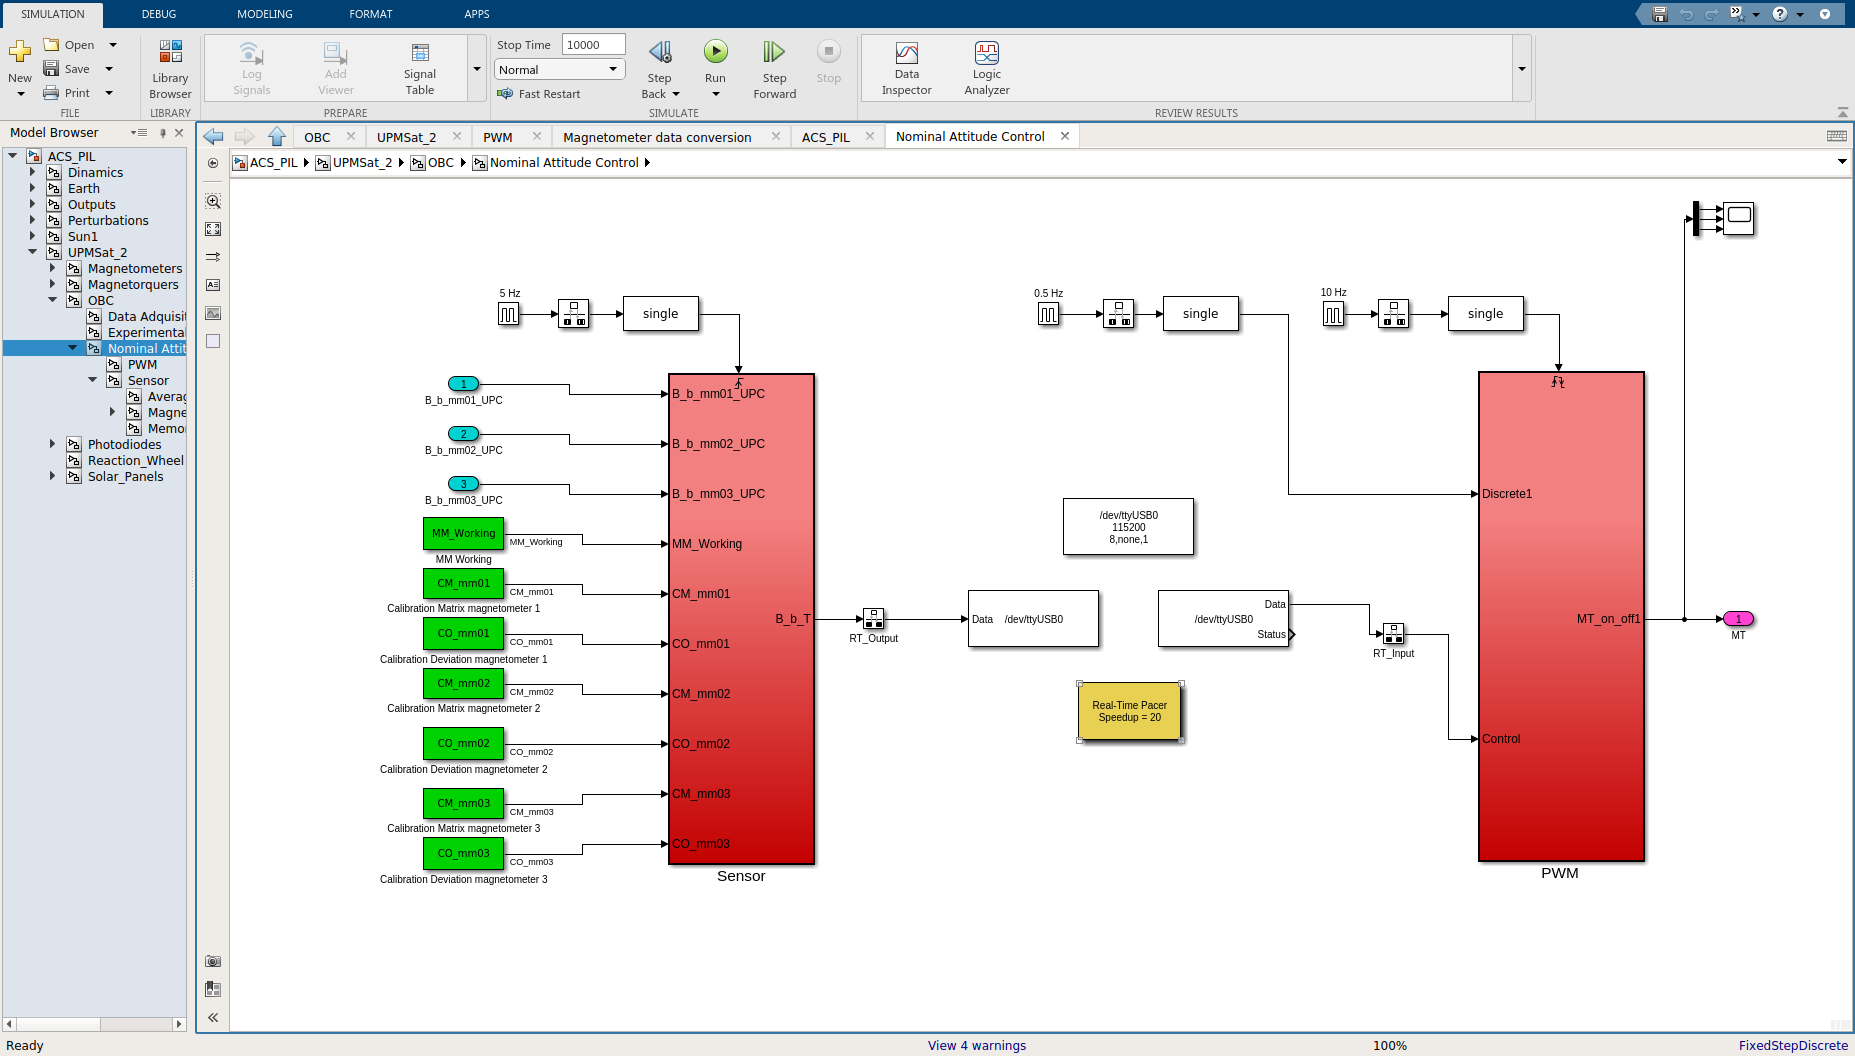
\includegraphics[width=\textwidth,keepaspectratio]{nac-pil.png}}
            \caption{Nominal attitude control for PIL.}
            \label{fig:nac-pil}
\end{figure}

Additional rate transition blocks has been added for a proper communication and a Real-Time Pacer block has been also added to set the simulation speed. In a real case, an speedup equal to 1 should be used but it is to slow.

Start the simulation and verify angular velocity stabilization. Now ADC runs and red LED is toggled. 

\section{Make changes to the simulation}

\begin{itemize}
\item Default parameters for control blocks can be changed in Ada source file ACS-parameters.ads.
\begin{itemize}
\item \texttt{Default\_omega} is the consigned angular velocity.
\item \texttt{Default\_MT\_Working} contains the operational magneto-torques.
\end{itemize}

In UPMSat-2 many parameters can be changed by TC.
\item The initial angular velocity can be changed in Simulink source file initialization.m.
\begin{itemize}
\item omega\_BI\_B0 = [0.1;-0.1;-0.1];
\end{itemize}
\end{itemize}

	\chapter{Documented report}

Students have to write a brief report of about 3-5 pages
on the work carried out during the session.
This report \textbf{must} include the following:

\begin{itemize}
	\item An analysis about cross-development environment for embedded systems and the main differences with a native environment.
	\item The schedulabilty analysis proposed in section~\ref{sc:ta}.
	\item The results from the ACS PIL simulation as shown in figure~\ref{fig:scope}.
	\item The report can contain recommendations to improve the assignment and personal opinions.
	\item A description of the changes proposed in the assignments (or any other), including the source code with comments.
\end{itemize}

All sections are mandatory, and the report must be uploaded in the designated assignment on the Moodle platform.
	%----------------------------------------------------------------------
	\cleardoublepage
	%%\addcontentsline{toc}{section}{\protect\textbf{Appendices}}
	\appendix
	%%\begin{appendices}
	%!TEX root = practica.tex
%===============================================================================
\chapter{Temperature sensor}\label{ap:sensor}
%\addcontentsline{toc}{chapter}{Temperature sensor}
%----------------------------------------------------------------------

The STM32F407 reference manual (section 13.10) states that the internal temperature sensor of the MCU is internally cabled to the ADC1\_IN16 analog input channel. The steps required to read the sensor are:

\begin{enumerate}
\item Select ADC1\_IN16 input channel in the ADC.
\item Select a sampling time greater than the minimum sampling time specified in the datasheet (see table~\ref{tb:sensor} below).
\item Set the TSVREFE bit in the ADC\_CCR register to wake up the temperature sensor from power down mode.
\item Start the ADC conversion by setting the SWSTART bit (or by external trigger).
\item Read the resulting VSENSE data in the ADC data register.
\item Calculate the temperature using the following formula:

Temperature (in \degree{C}) = {(VSENSE - V25) / Avg\_Slope} + 25

Where:
\begin{itemize}
\item V25 = VSENSE value for 25 \degree{C} (table~\ref{tb:sensor})
\item Avg\_Slope = average slope of the temperature vs. VSENSE curve (table~\ref{tb:sensor}).
\end{itemize}
\end{enumerate}

The sensor has a startup time after waking from power down mode before it can output VSENSE at the correct level. The ADC also has a startup time after power-on, so to minimize the delay, the ADON and TSVREFE bits should be set at the same time.

The sensor has a range of -40 to 125 \degree{C}, with a precision of $\pm$1.5 \degree{C}. Its main characteristics are described in the STM32F407 datasheet (table~\ref{tb:sensor}).

\begin{table}[htb]
\begin{center}
\begin{tabular}{llllll} \hline
Symbol & Parameter & Min & Typ & Max & Unit \\ \hline
TL & VSENSE linearity with temperature & - & $\pm1$ & $\pm2$ & \degree{C}\\
Avg\_Slope & Average slope & - & 2.5 & & mV/\degree{C}\\
V25 & Voltage at 25 \degree{C} & - & 0.76 & & V\\
tSTART & Startup time & - & 6 & 10 & $\mu{s}$\\
TS\_temp & ADC sampling time when reading & 10 & - & - & $\mu{s}$\\
& the temperature (1 \degree{C} accuracy) &  &  &  & \\ \hline
\end{tabular}
\caption{STM32F407 temperature sensor characteristic.}
\label{tb:sensor}
\end{center}
\end{table}

The Ada Drivers Library includes the package STM32.ADC, which provides facilities for handling the analog to digital converter.

	%%\end{appendices}
	%======================= back matter ===================================
	%\addcontentsline{toc}{chapter}{\numberline{}Bibliography}
	%\bibliography{realtime,anser}
	%\cleardoublepage
\end{document}

